% This is a LaTeX thesis template for Monash University.
% to be used with Rmarkdown
% This template was produced by Rob Hyndman
% Version: 6 September 2016

\documentclass{monashthesis}

%%%%%%%%%%%%%%%%%%%%%%%%%%%%%%%%%%%%%%%%%%%%%%%%%%%%%%%%%%%%%%%
% Add any LaTeX packages and other preamble here if required
%%%%%%%%%%%%%%%%%%%%%%%%%%%%%%%%%%%%%%%%%%%%%%%%%%%%%%%%%%%%%%%

\usepackage{thumbpdf,lmodern}
\usepackage{amsmath}
\usepackage{bm}
\usepackage{booktabs}
%%%% NS
\usepackage{graphicx}
%\usepackage{pdflscape} %% Allow landscape layout, not used
%\usepackage{lmodern} %% Already loaded, allows GB Pound sign
\usepackage{animate} %% Needed for animations
\PassOptionsToPackage{hyphens}{url}\usepackage{hyperref} %% Trying to wrap and format urls correctly


\author{Nicholas S Spyrison}
\title{Dynamic visualization of high-dimensional data via low-dimension projections, their efficay, and their application to model-agnostic local explanations}
\degrees{B.Sc. Statistics, Iowa State University}
\def\degreetitle{Doctor of Philosophy}
% Add subject and keywords below
\hypersetup{
     %pdfsubject={The Subject},
     %pdfkeywords={Some Keywords},
     pdfauthor={Nicholas S Spyrison},
     pdftitle={Dynamic visualization of high-dimensional data via low-dimension projections, their efficay, and their application to model-agnostic local explanations},
     pdfproducer={Bookdown with LaTeX}
}


\bibliography{thesisrefs}

\begin{document}

\pagenumbering{roman}

\titlepage

{\setstretch{1.2}\sf\tighttoc\doublespacing}

\hypertarget{abstract}{%
\chapter*{Abstract}\label{abstract}}
\addcontentsline{toc}{chapter}{Abstract}

Visualizing data space is crucial to exploratory and general data analysis yet doing so quickly becomes difficult as the dimensionality of the data increases. Traditionally, static, low-dimensional linear embeddings are used to identify clustering, outliers, and structure. Observing one such embedding often misses a significant amount of variation, and hence, information held within the data. \emph{Tours} are a class of dynamic linear projections that animates many linear projections as the orientation in data space changes. User-controlled steering (UCS) of the original dimensionality offers fine control of the local structure of projections.

Data visualization has lagged behind in utilizing 3D and virtual spaces after the overhype of the 1980s and '90s gave way to some unpromising results. Modern mixed reality hardware has significantly improved the quality and simultaneously reduced the barrier to entry. Contemporary studies have regularly shown increased accuracy of perception of visuals displayed in 3D over 2D, including in projected subspaces. It's time to further explore dynamic projections in virtual spaces.

Multivariate data is ubiquitous and viewing it in data-space is a crucial aspect of data analysis and consumption. This research is four-fold and allows for fine exploration of the data structure in embeddings of high dimensional spaces, contrasts UCS with traditional static techniques, extends UCS \& creates surface projections in 3D space, and quantifies the benefits of dynamic projections across display devices.

\clearpage\pagenumbering{arabic}\setcounter{page}{0}

\hypertarget{ch:introduction}{%
\chapter{Introduction}\label{ch:introduction}}

\hypertarget{exploratory-data-analysis}{%
\section{Exploratory data analysis}\label{exploratory-data-analysis}}

The term exploratory data analysis was coined in \textcite{tukey_exploratory_1977}, who leaves it as an intentionally broad term wich encompass the initial summarization and visualization of a data set. This is a critical first step of checking for realistic values and validating assumptions made by prospective methodology. Visualization is crucial to a clear understanding of the data. Things can go awry when data is summarized via numeric statistics alone \autocite{anscombe_graphs_1973} as demonstrated in figure \ref{fig:matejka17fig} \autocite{matejka_same_2017}. In these studies, bivariate data have the same summary statistics (such as mean and standard deviation), yet contains obvious visual trends and shapes that could go completely unheeded if plotting is foregone. Because there are inherent dangers to relying on statistics alone, this requirement for looking at visuals necessitates \emph{human-in-the-loop} analysis, defined as any model that requires human interaction \autocite{karwowski_international_2006}.



\begin{figure}

{\centering 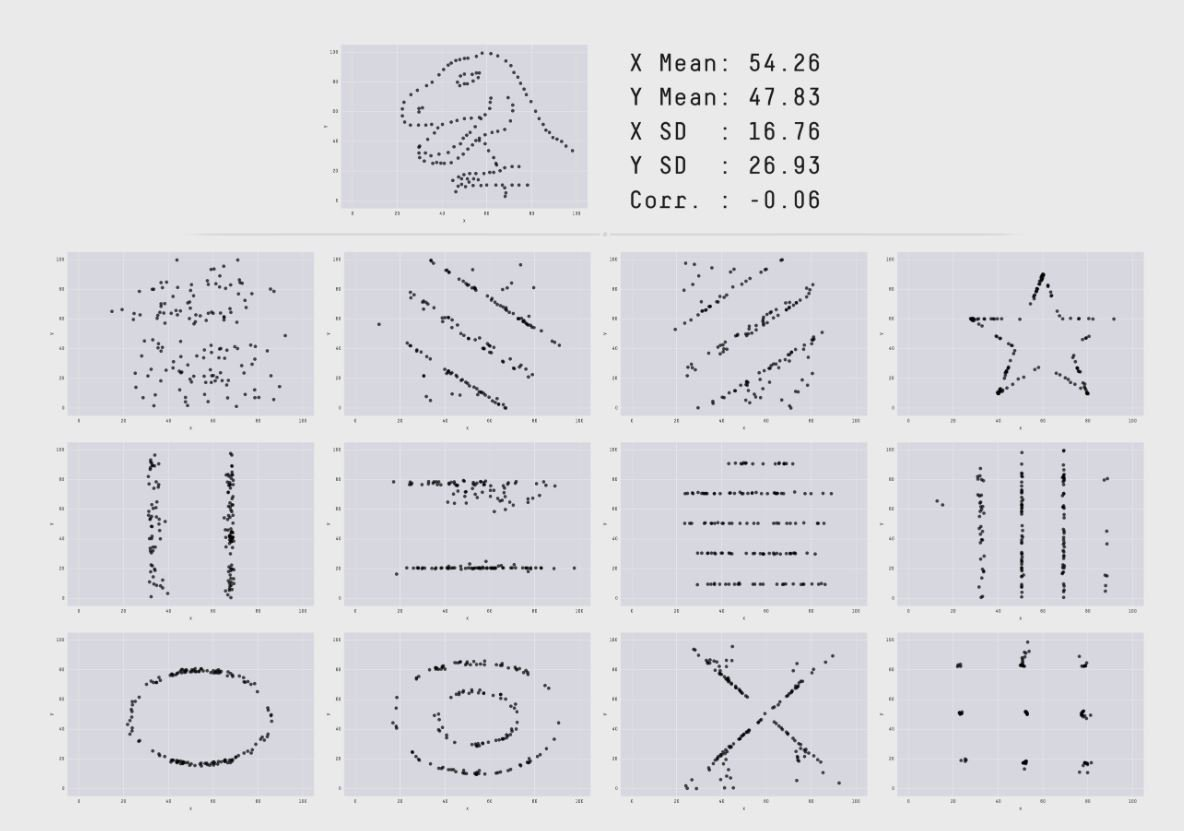
\includegraphics[width=0.7\linewidth]{./figures/matejka17fig} 

}

\caption{12 data sets created from the datasaurus by simulated annealing. Each is restrained to the same summary statistics but given shapes with visual peculiarity to mutate into \autocite{matejka_same_2017}.}\label{fig:matejka17fig}
\end{figure}

It is clear that data-space visualization is needed but it becomes complex as data dimensionality increases. Embedding (or projecting) \(p-\)dimensional data on to a lower, \(d\)-dimensional subspace is a common dimension reduction approach to visualize multivariate data spaces. Traditionally a single static projection is used to summarize a space, which necessarily shows a subset of the variation of the data. \textcite{asimov_grand_1985} suggested the use of viewing projections dynamically across a changing projection basis allows for more variation to be contained and viewed temporally. This dynamic view of many changing projections is known as \emph{tours}. While, there are different methods of generating tour paths, human-in-the-loop user-controlled steering (UCS) offers the finest control for navigating the local structure.

Tours are typically viewed from standard 2D monitors, and most commonly viewed as a projection down to 2D. A notable exception being \textcite{nelson_xgobi_1998}, where 3D embeddings were viewed in 3D head-tracked VR. Data visualization studies generally show benefits in 3D visuals over 2D, especially when adequate depth cues are provided. The state of modern hardware has made VR more affordable and available to wider audiences, at ever increasing resolutions of display than previously possible. It is therefore timely for research to be conducted to compare the structure and speed of comprehension of dynamic linear projections across 2- and 3D display devices.

\hypertarget{research-objectives}{%
\section{Research objectives}\label{research-objectives}}

Data and models are typically high-dimensional, with many variables and parameters. Developing new methods to visualize high dimensions has been a pursuit of statisticians, computer scientists and visualization researchers for decades. As technology evolves examining, extending, and assessing current techniques, in new environments, for new data challenges, is an important endeavor. The primary objectives of this Ph.D.~research can then be summarized as the following.

\textbf{Research objectives (RO):}

\begin{enumerate}
\def\labelenumi{\arabic{enumi}.}
\item
  \textbf{How can UCS be generalized to work within graphic-specific environments for 2D projections?}\\
  (Work in progress, chapter \ref{ch:workinprogress}.)\\
  Building from the UCS algorithm in \textcite{cook_manual_1997}, the algorithm should be modified for generalized use with graphic-specific environments. This enables fine control to explore the sensitivity of structure to the variable contributing to the projection and sets the foundation to be used in the remaining objectives.
\item
  \textbf{Does 2D UCS tours provide benefits over alternatives?}\\
  (Future work, chapter \ref{ch:future_work}.)\\
  The quality and effectiveness of 2D UCS will be compared with alternatives of static, single, linear and non-linear projection techniques. They will be quantified by the measurement of structure, variation, and clustering across on benchmark datasets.
\item
  \textbf{How can UCS be extended to 3D?}\\
  (Future work, chapter \ref{ch:future_work}.)\\
  The addition of a 3rd dimension potentially allows for the improved perception of the structure of the data in dynamic UCS. To investigate this UCS algorithm needs to be extended to a third dimension. This would also allow for novel application multi-parameter function projection. This will involve the addition of a new angle and it controls to the projection space, reference axes, and manipulation space. In particular, the manipulation space, now in 4D, will be hard to visualize, but it should be able to stand as a mathematical construct facilitated through interaction with a point (the projection coefficients of the selected manipulation variable) on the now 3D reference axes volume.
\item
  \textbf{Does UCS in 3D displays provide benefits over 2D displays?}\\
  (Future work, chapter \ref{ch:future_work}.)\\
  The addition of a 3rd dimension has previously been shown to provide benefits. The extension of UCS into 3D should be used to explore the potential benefits of UCS projections as well. Interactive, time-varying tours theoretically allow for improved understanding and comprehension speed of the structure of the data. These metrics will be measured across the display device (including a 2D standard monitor, 3D head tracked monitor, and 3D head-mounted display).
\end{enumerate}

\textbf{Contributions:}

The intended contributions and scope of this research can be summarized as:

\begin{enumerate}
\def\labelenumi{\arabic{enumi}.}
\tightlist
\item
  A modified UCS algorithm and new implementation applied to contemporary high energy physics and astrophysics applications in 2D animation frameworks.
\item
  A performance comparison of static and interactive UCS projection techniques assessed on benchmark data sets from the recent literature.
\item
  A new algorithm for UCS in 3D. With new applications to function visualization in 3D.
\item
  Quantitative understanding of the relative benefits of UCS across 2- and 3D display devices.
\end{enumerate}

\hypertarget{methodology}{%
\section{Methodology}\label{methodology}}

This research is interdisciplinary; it stems from a linear dimension reduction technique developed by statisticians and extended with information technology into 3D including VR technologies, with applications in high energy physics identified\autocite{cook_dynamical_2018}. Experts in these fields correspondingly supervise the research.

The research corresponding with RO \#1 entails a work in progress \textbf{algorithm design} following the work in \textcite{cook_manual_1997}. The proposed algorithm discusses the generalized application of UCS for use across animation-specific frameworks. The outcome of this is an \emph{R} package, \texttt{spinifex}, which will be submitted to CRAN and for hosting and distribution. This forms the foundation for future work in the remaining objectives.

The second objective is addressed with a benchmark dataset \textbf{performance comparison} between dynamic linear projections and alternatives (static linear and static non-linear projections such as principal component analysis, multi-dimensional scaling, and t-distributed neighbor embeddings, described in more detail in chapter \ref{ch:future_work}). Benchmark datasets will be compared across techniques, measurements will include variation explained, transparency to the original variable space, clustering identification, and outlier identification.

The research for RO \#3 involves \textbf{algorithm design}, where the work in RO \#1 will be extended to display with the use of a third spatial dimension. This will also be used to develop visualization of projected multi-dimension function surfaces. This forms the calculation base for the work. Several difficulties may arise when bringing dynamic projection into 3D spaces, especially when exploring 3D surfaces (discussed in more detail in chapter \ref{ch:future_work}).

The research resulting from RO \#4 is a controlled \textbf{usability study} to explore the efficacy of bringing UCS into 3D as compared across various display devices, in a standardized interface allowed by the work stemming from RO \# 3. In this design, the factors are user tasks (such as separation of clusters and ranking of manipulation variable) across the treatment of display device (including 2D standard monitor, 3D head-tracked monitor, and head-mounted display). Quantitative measurements include participant speed and accuracy of tasks, biometric readings, and subjective Likert surveys of participants. A lineup-type model as outlined in \textcite{hofmann_graphical_2012} may also be employed for assessing the quality of display types.

\hypertarget{workflow-and-reproducibility}{%
\section{Workflow and reproducibility}\label{workflow-and-reproducibility}}

Figure \ref{fig:dataanalysisworkflow} depicts the general data analysis workflow \autocite{wickham_r_2016}. Where data first must be imported into a tool, the structure of the data must be tidied and ordered neatly into the correct use format. After the data enters a repeating cycle, where values may be transformed, visualized, and modeled with communication going to the appropriate recipients. The research proposed in this document aids exploratory data analysis as well as the visualization aspect of this workflow. Mature analysis workflow is also made reproducible with the use of programmatic scripts.



\begin{figure}

{\centering 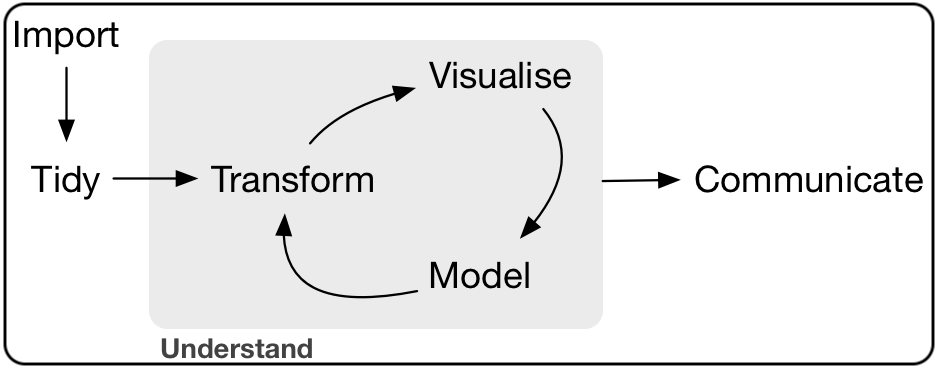
\includegraphics[width=1\linewidth]{./figures/data_analysis_workflow} 

}

\caption{Data analysis workflow \autocite{wickham_r_2016}. This research aids visualization in exploratory data analysis and workflow.}\label{fig:dataanalysisworkflow}
\end{figure}

The programing language, \emph{R}, is used in the work described below to import, tidy, and transform data. It can be used directly to visualize 2D tours (RO \#1 \& 2) or be consumed into the game engine \emph{Unity} to visualize 3D tours (RO \#3 \& 4). Doing analysis and writeup in such programmatic ways allow work to be done reproducibly. Where data, analysis, and code are stored in the same directory. Reproducible work facilitates validation, maintains transparency and minimizes the chance for human error. Reproduction of work is a key feature to validate and defend the claims and methodology held within a work. Directories of current and planned work are/will be hosted publicly on GitHub, including this report. Accessing the source files for this report is discussed in section \ref{sec:source}.

\hypertarget{ch:projectoverview}{%
\section{Project overview}\label{ch:projectoverview}}

Figure \ref{fig:ProjectOverview} depicts a schematic flow chart that the research objectives will be executed in. The research stemming from RO \#1, the application of 2D user-controlled steering (UCS), sets the foundation for which the other objectives can be researched. RO \#3, the application of 3D UCS, must precede RO \#4, as it explores the efficacy of 3D UCS across display devices. RO \#2, the comparison of 2D UCS vs alternatives, must come after RO \#1, but is of lower priority to RO \#3 \& 4, and so will be conducted last, in the event of a time crunch.



\begin{figure}

{\centering \includegraphics[width=1\linewidth]{./figures/ProjectOverview} 

}

\caption{Flow chart of research objective dependencies, work order, and methodology.}\label{fig:ProjectOverview}
\end{figure}

In this report, the related literature is discussed in chapter \ref{ch:lit_review}. A brief overview of the research is given in chapter \ref{ch:projectoverview}, followed by ongoing work and future work in chapters \ref{ch:workinprogress} and \ref{ch:future_work} respectively. A prospective timeline is listed in chapter \ref{ch:timeline}. Notation for dynamic projections and VR data visualization can be found in appendix \ref{ch:glossary} and an excerpt of a paper to be submitted to the R Journal can be found in appendix \ref{ch:spinifex}.

\hypertarget{ch:lit_review}{%
\chapter{Literature review}\label{ch:lit_review}}

The following chapter discusses the current research in two primary areas: dynamic linear projections (collectively known as tours) and multivariate data visualization in stereoscopic 3D. After each section, research gaps are highlighted.

\hypertarget{sec:tour}{%
\section{Dynamic linear projections of multivariate data (tours)}\label{sec:tour}}

\hypertarget{overview}{%
\subsection{Overview}\label{overview}}

The introduction established that visualizing data-space is an important aspect of exploratory data analysis and data analysis in general. Yet, there is an inherent difficulty as the dimensionality of data increases. In univariate data sets histograms or smoothed density curves are employed to visualize data. In bivariate data, \(XY\) scatterplots and contour plots (2D density) can be employed. In three dimensions, the two most common techniques are 3D scatterplot\footnote{Graphs depicting three dimensions are typically viewed on a 2D display, in print or with a standard monitor. These are 2D images of monocular 3D spaces, sometimes referred to as 2.5D data visualization, more on this in section \ref{sec:3d-terminology}.} or 2D scatterplot with the 3rd variable as an aesthetic (such as color, size, or height). These aesthetic cues convey some information but are not a sufficient replacement for axes for use with continuous variables.

As dimensionality of the data, \(p\), increases the visualization of data-space quickly becomes complex. It is common that visualizing data-space is dropped in favor of graphing model-space (for example residuals), parameter-space (in fewer dimensions), or worse yet: long tables of statistics without visuals \autocite{wickham_visualizing_2015}. To preserve the visualization of data-space, a solution that scales with the dimensionality of data is needed; this is where dimensionality reduction comes in. This work will focus on a group of dynamic linear projection techniques collectively known as \emph{tours}. The scope of the project lies within the dynamic linear projections; a broader review of dimensionality reduction techniques is discussed in the review paper by \textcite{grinstein_high-dimensional_2002}. Tours are used for a couple of salient features: the use of linear projections maintains transparency back to the original variable space (which non-linear projections lose) and the use of many projections shows more variation than a single linear projection. Employing the breadth of tours extends the dimensionality of visualizations, and with it, the intrinsic understanding of the structure and distribution of data that is more succinct or beyond the reach of summary statistics alone.

Let \(p\) be the dimensionality of the data, and \(d\) be the dimension of the projection space. Tours perform linear dimensionality reduction, orthogonally projecting \(p\)-space down to \(d(\leq p)\) dimensions. Many such projections are interpolated, each making small rotations in \(p\)-space. These frames are then viewed in order as an animation of the lower dimensional embedding changing as the original variable space is manipulated. Shadow puppets offer a useful analogy to aid in conceptualizing tours. Imagine a fixed light source facing a wall. When an object is introduced it projects a 2D shadow onto the wall. This is a physical representation of a simple projection, that from \(p=3\) down to \(d=2\). If the object rotates then the shadow correspondingly changes. Observers watching only the shadow are functionally watching a 2D tour as the 3D object is manipulated. Some orientations explain more information about the shape of the object than others while watching an animation of the shadow changing gives a more robust understanding than looking at any one frame. More complex structures generally require more time to comprehend the nature of the geometry. These features hold for tours as well.

\emph{An extended tour notation is listed in the appendix section \ref{sec:tour_notation}.}

\hypertarget{history}{%
\subsection{History}\label{history}}

The first tour was introduced was the \emph{grand tour} in \textcite{asimov_grand_1985} at the Stanford Linear Accelerator, Stanford University. Asimov suggested three types of grand tours: torus, at-random, and random-walk. The original application of tours was performed on high energy physics on the PRIM-9 system.

Before choosing projection paths randomly, an exhaustive search of \(p-\)space was suggested by \textcite{mcdonald_interactive_1982}, also at the Stanford Linear Accelerator. This was later coined \emph{little tour}.

\textcite{friedman_projection_1974} and later \textcite{huber_projection_1985} recommended projection pursuit (also referred to as PP). Projection pursuit optimizes an objective function before it removes a single component/variable and then iterates in this newly embedded subspace. Within each subspace, the projection seeks for a local extremum via a hill climbing algorithm on an objective function. This formed the basis for \emph{guided tours} suggested by \textcite{hurley_analyzing_1990}.

The grand and little tours have no input from the user aside from the starting basis. Guided tours allow for an index to be selected. The bulk of tour development since has largely been around the dynamic display, user interaction, geometric representation, and application.

\hypertarget{sec:path_generation}{%
\subsection{Path generation}\label{sec:path_generation}}

A fundamental aspect of tours is the path of rotation. There are four primary distinctions of tour path generation \autocite{buja_computational_2005}: random choice, data-driven, precomputed choice, and manual control.

\begin{itemize}
\tightlist
\item
  Random choice, \emph{grand tour}, constrained random walks \(p\)-space. Paths are constrained for changes in direction small enough to maintain continuity and aid in user comprehension

  \begin{itemize}
  \tightlist
  \item
    torus-surface \autocite{asimov_grand_1985}
  \item
    at-random \autocite{asimov_grand_1985}
  \item
    random-walk \autocite{asimov_grand_1985}
  \item
    \emph{local tour} \autocite{wickham_tourr_2011}, a sort of grand tour on a leash, such that it goes to a nearby random projection before returning to the original position and iterating to a new nearby projection.
  \end{itemize}
\item
  Data-driven, \emph{guided tour}, optimizing some objective function/index within the projection-space, called projection pursuit (PP) \autocite{hurley_analyzing_1990}, including the following indexes:

  \begin{itemize}
  \tightlist
  \item
    holes \autocite{cook_projection_1993} - moves points away from the center.
  \item
    cmass \autocite{cook_projection_1993} - moves points toward the center.
  \item
    lda \autocite{lee_projection_2005} - linear discriminant analysis, seeks a projection where 2 or more classes are most separated.
  \item
    pda \autocite{lee_projection_2010} - penalized discriminant analysis for use in highly correlated variables when classification is needed.
  \item
    convex \autocite{laa_using_2019} - the ratio of the area of convex and alpha hulls.
  \item
    skinny \autocite{laa_using_2019} - the ratio of the perimeter distance to the area of the alpha hull.
  \item
    stringy \autocite{laa_using_2019} - based on the minimum spanning tree (MST), the diameter of the MST over the length of the MST.
  \item
    dcor2D \autocite{grimm_mbgraphic:_2017,laa_using_2019} - distance correlation that finds linear and non-linear dependencies between variables.
  \item
    splines2D \autocite{grimm_mbgraphic:_2017,laa_using_2019} - measure of non-linear dependence by fitting spline models.
  \item
    other user-defined objective indices can be applied to the framework provided in the \emph{tourr} package \textcite{wickham_tourr_2011}.
  \item
    Another data-drive tour is the \emph{dependence tour}, a combination of \(n\) independent 1D tours. A vector describes the axis each variable will be displayed on. for example \(c(1, 1, 2, 2)\) is a 4- to 2D tour with the first 2 variables on the first axis, and the remaining on the second.

    \begin{itemize}
    \tightlist
    \item
      \emph{correlation tour} \autocite{buja_data_1987}, a special case of the dependence tour, analogous to canonical correlation analysis.
    \end{itemize}
  \end{itemize}
\item
  Precomputed choice, \emph{planned tour}, in which the path has already been generated or defined.

  \begin{itemize}
  \tightlist
  \item
    \emph{little tour} \autocite{mcdonald_interactive_1982}, where every permutation of variables is stepped through in order, analogous to brute-force or exhaustive search.
  \item
    a saved path of any other tour, typically an array of basis targets to interpolate between.
  \end{itemize}
\item
  Manual control, \emph{manual tour}, a constrained rotation on selected manipulation variable and magnitude \autocite{cook_manual_1997}. Typically used to explore the local area after identifying an interesting feature, perhaps via guided tour.
\end{itemize}

\hypertarget{path-evaluation}{%
\subsection{Path evaluation}\label{path-evaluation}}

Consider projection down to 2D, then each projection is called a 2-frame (each spanning a 2-plane). Mathematically, a Grassmannian is the set of all possible unoriented 2-frames in \(p\)-space, \(\textbf{Gr}(2,~p)\). \textcite{asimov_grand_1985} pointed out that the unique 2-frames of the grand tour approaches \(\textbf{Gr}(2,~p)\) as time goes to infinity. The \emph{density} of a tour is defined as the fraction of the Grassmannian explored. Ideally, an exploring tour will be dense, but the time taken to become dense vastly increases as variable space increases dimensionality. \emph{Rapidity} is then defined as how quickly a tour encompasses the Grassmannian. Due to the random selection of a grand tour, it will end up visiting homomorphisms of previous 2-frames before all unique values are visited, leading sub-optimal rapidity.

The little tour introduced in \textcite{mcdonald_interactive_1982}, on the other hand, is necessarily both dense and rapid, performing essentially an exhaustive search on the Grassmannian. However, this path uninteresting and with long periods of similar projections strung together. The Grassmannian is necessarily large and increases exponentially at the rate of \(p\). Viewing of the whole Grassmannian is time-consuming, and interesting projections are sparse, there was a clear space for computers to narrow the search space.

Guided tours \autocite{hurley_analyzing_1990} optimize an objective function generating path will be a relatively small subset of the Grassmannian. As they are not used for exploration, density and rapidity are poor measures. On the other hand, they excel at finding interesting projections quickly. Recently, \textcite{laa_using_2019}, compared projection pursuit indices with the metrics: \emph{smoothness, squintability, flexibility, rotation invariance} and \emph{speed}.

\hypertarget{sec:geom_display}{%
\subsection{Geometric display by dimensionality}\label{sec:geom_display}}

Up to this point, 2D scatterplots have been the primary display discussed, they offer a logical display for viewing embeddings of high-dimensional point clouds. However, other geometrics offer perfectly valid projections as well.

\begin{itemize}
\tightlist
\item
  1D geometrics (geoms)

  \begin{itemize}
  \tightlist
  \item
    1D densities: such as histogram, average shifted histograms \autocite{scott_averaged_1985}, and kernel density \autocite{scott_incorporating_1995}.
  \item
    image (pixel): \autocite{wegman_pixel_2001}.
  \item
    time series: where multivariate values are independently lagged to view peak and trough alignment. Use case is discussed in \autocite{cook_manual_1997}.
  \end{itemize}
\item
  2D geoms

  \begin{itemize}
  \tightlist
  \item
    2D density (available on GitHub at \url{https://github.com/nspyrison/tourr})
  \item
    \(XY\) scatterplot
  \end{itemize}
\item
  3D geoms

  \begin{itemize}
  \tightlist
  \item
    Anaglyphs, sometimes called stereo, where red images are positioned for the left channel and cyan for the right when viewed with corresponding filter glasses give a perception of depth to the image.
  \item
    Depth, which gives depth cues via aesthetic mappings, most common size and/or color of data points.
  \end{itemize}
\item
  \(d\)-dimensional geoms

  \begin{itemize}
  \tightlist
  \item
    Andrews curves \autocite{andrews_plots_1972}, smoothed variant of parallel coordinate plots, discussed below.
  \item
    Chernoff faces \autocite{chernoff_use_1973}, variables linked to the size of facial features. The idea is to apply the human facial-perception for rapid, cursory, like-ness comparisons between observations.
  \item
    Parallel coordinate plots {[}\textcite{ocagne_coordonnees_1885}; wegman\_hyperdimensional\_1990{]}, where any number of variables are plotted in parallel with observations linked to their corresponding variable value by polylines.
  \item
    Scatterplot matrix (SPLOM) \autocite{chambers_graphical_1983}, showing a triangle matrix of bivariate scatterplots with 1D density on the diagonal.
  \item
    Radial glyphs, radial variants of parallel coordinates including radar, spider \autocite{duffin_spiders:_1994}, and star glyphs \autocite{siegel_surgical_1972}.
  \end{itemize}
\end{itemize}

\hypertarget{tour-software}{%
\subsection{Tour software}\label{tour-software}}

Tours have yet to be widely adopted, due in part, to the fact that print and static .pdf output does not accommodate dynamic viewing. Conceptual abstraction and technically density have also hampered user growth. Due to low levels of adoption and the rapid advancement of technology support and maintenance of such implementations give them a particularly short life span. Despite the small user base, there have been a fair number of tour implementations, including:

\begin{itemize}
\tightlist
\item
  spinifex \href{https://github.com/nspyrison/spinifex}{github.com/nspyrison/spinifex} -- R package, all platforms.
\item
  tourr \autocite{wickham_tourr_2011} -- R package, all platforms.
\item
  CyrstalVision \autocite{wegman_visual_2003} -- for Windows.
\item
  GGobi \autocite{swayne_ggobi:_2003} -- for Linux and Windows.
\item
  DAVIS \autocite{huh_davis:_2002} -- Java based, with GUI.
\item
  ORCA \autocite{sutherland_orca:_2000} -- Extensible toolkit built in Java.
\item
  VRGobi \autocite{nelson_xgobi_1998} -- for use with the C2, tours in stereoscopic 3D displays.
\item
  ExplorN \autocite{carr_explorn:_1996} -- for SGI Unix.
\item
  ExploRe \autocite{hardle_xplore:_1995}
\item
  XGobi \autocite{swayne_xgobi:_1991} -- for Linux, Unix, and Windows (via emulation).
\item
  XLispStat \autocite{tierney_lisp-stat:_1990} -- for Unix and Windows.
\item
  Explor4 \autocite{carr_explor4:_1988} -- Four-dimensional data using stereo-ray glyphs.
\item
  Prim-9 \autocite{asimov_grand_1985,fisherkeller_prim-9:_1974} -- on an internal operating system.
\end{itemize}

\hypertarget{research-gaps}{%
\subsection{Research gaps}\label{research-gaps}}

Dynamic projections offering UCS have not incorporated recent animation frameworks (\textbf{RO \#1}). This leaves the class of dynamic linear projections without the most precise, fine-scale control of rotating \(p\)-space. This should be implemented with an eye on extensibility and maintainability.

A comparative study outlining the benefits of UCS vs alternatives is also absent from the literature (\textbf{RO \#2}). The benefits of dynamic linear projections hold in theory, but a direct comparison with popular alternatives should be made. Barriers to adoption and sharing should also be kept in mind as the dynamic display is not easy to display on print and in .pdf documents.

\hypertarget{sec:3d}{%
\section{Multivariate data visualization in 3D}\label{sec:3d}}

The scope of this research pertains to numeric multivariate data, a wider overview of 3D data visualization is discussed in chapter 2 of \textcite{marriott_immersive_2018}. Terminology for 3D visuals is in the glossary section \ref{sec:3d-terminology}.

\hypertarget{a-rocky-start}{%
\subsection{A rocky start}\label{a-rocky-start}}

Scientific visualization has readily adopted mixed realities as a large amount of the science exists in three spatial dimensions, lending itself well to virtual immersion \autocite{marriott_immersive_2018}. Data visualization, on the other hand, has been slow to utilize graphics above 2.5D, (and haptic interaction) primarily due to the mixed results of over-hyped of 3D visuals from the 1980s and '90s \autocite{munzner_visualization_2014}. Since then, however, there have been several promising studies suggesting that it is time for data visualization to revisit and adopt the use of 3D visuals for specific combinations of displays and depth cues.

\hypertarget{d-rotated-projections-vs-3-2d-orthogonal-projections}{%
\subsection{3D rotated projections vs 3 2D orthogonal projections}\label{d-rotated-projections-vs-3-2d-orthogonal-projections}}

Three orthogonal 2D views can represent the three face-on views of 3D shapes. When 3D representations are used with binocular cues, they are found to have more accurate perception than 2D counterparts \autocite{lee_effects_1986}.

Between 3D and split view 2D of three-dimensional economics, data \textcite{wickens_implications_1994} asked participants questions integrating several variables, finding that 3D visuals resulted in faster answers when questions involved three dimensions, while the speed was similar when questions involved fewer dimensions.

Using 3D rotated projections gives more precise (relative to 2D) estimates of the height a ball is suspended above complex box shapes, while combinations of 2D and 3D give the most precise orientation and positioning information \autocite[depicted in figure \ref{fig:tory06fig}]{tory_visualization_2006}.



\begin{figure}

{\centering \includegraphics[width=0.5\linewidth]{./figures/tory06fig} 

}

\caption{Screen capture from \textcite{tory_visualization_2006}: ``fig.~1 (a) 2D, (b) 3D Rotated, (c) 3D Shadow, (d) Orientation Icon, and (e) ExoVis displays used in Experiment 1 (position estimation). Participants estimated the height of the ball relative to the block shape. In this example, the ball is at height 1.5 diameters above the block shape.''}\label{fig:tory06fig}
\end{figure}

\textcite{sedlmair_empirical_2013}, depicted in figure \ref{fig:sedlmair13fig}, asked users about cluster separation across 2D scatterplots, 2D scatterplot matrices (SPLOMs) and interactive 3D scatterplots, PCA (linear projection), and t-SNE (non-linear projection) as viewed in monocular 3D from a standard monitor. They conclude that interactive 3D scatterplots perform worse for class separation. This result is surprising as the extra dimension theoretically allows for the clustering structure to be seen and explored more clearly.



\begin{figure}

{\centering \includegraphics[width=1\linewidth]{./figures/sedlmair13fig} 

}

\caption{Screen capture of ``figure 5. example of a mesh display'' from \textcite{sedlmair_empirical_2013}: ``fig.~5. (a)-(d): Screenshots of the entangled dataset \texttt{entangled1-3d-3cl-separate} designed to show the most possible benefits for i3D. (a),(b) two viewpoints of the same i3D PCA scatterplot. An accompanying video shows the full 3D rotation. (c) 2D PCA projection. (d) t-SNE untangles this class structure in 2D. (e)-(f): 2D scatterplots of the reduced \texttt{entangled2-15d-adjacent} dataset which we designed to have a ground truth entangled class structure in 15D. (e) Glimmer MDS cannot untangle the classes, neither can PCA and robPCA (see supplemental material). (f) t-SNE nicely untangles and separates the ground truth classes in 2D.''}\label{fig:sedlmair13fig}
\end{figure}

\hypertarget{comparing-3d-and-2d-embeddings-of-multivariate-data}{%
\subsection{Comparing 3D and 2D embeddings of multivariate data}\label{comparing-3d-and-2d-embeddings-of-multivariate-data}}

\textcite{nelson_xgobi_1998}, depicted in figure \ref{fig:nelson98fig}, had \(n=15\) participants perform brushing and identification tasks (of clusters, structure, and data dimensionality) in 3D with head-tracked binocular VR. 3D proved to have a substantial advantage for cluster identification and some advantage in identifying the shape. Brushing did take longer in VR, perhaps due to the lower familiarity of manipulating 3D spaces.



\begin{figure}

{\centering \includegraphics[width=0.7\linewidth]{./figures/nelson98fig} 

}

\caption{Screen capture from \textcite{nelson_xgobi_1998}: ``figure 4: This is a picture of a 3-D room, running VRGobi. Data is plotted in the center, with painting tools to the right and variable spheres to the left. In the viewing box, the data can be seen to contain three clusters, and one is being brushed.''}\label{fig:nelson98fig}
\end{figure}

Another study, \textcite{gracia_new_2016} performed dimensionality reduction down to 2- and 3D scatterplots, both displayed in monocular 3D on a standard monitor. Users were found to more accurately compare distances between points and identify outliers on 3D scatterplots. However, both tasks were performed slower with the use of the 3D scatterplots and statistical significance was not reported.

\textcite{wagner_filho_immersive_2018}, depicted in figure \ref{fig:wagner18fig}, performed an \(n=30\) empirical study on PCA embedded projections, measuring perception error across 4 tasks and 3 display types: 2D, static 3D, and immersive 3D. Overall task error was less in static and immersive 3D relative to 2D. According to the user Likert-scale survey, 2D is slightly easier to navigate and slightly more comfortable, while, static and immersive 3D displays are slightly easier to interact with and moderately easier to find information on.



\begin{figure}

{\centering \includegraphics[width=0.5\linewidth]{./figures/wagner18fig} 

}

\caption{Screen capture from \textcite{wagner_filho_immersive_2018}, original captions contained in the capture.}\label{fig:wagner18fig}
\end{figure}

\hypertarget{immersive-analytics-platform-in-vr}{%
\subsection{Immersive analytics platform in VR}\label{immersive-analytics-platform-in-vr}}

Immersive analytics is an emerging field, where data visualization and analysis is facilitated in an intuitive, immersive virtual reality environment \autocite{chandler_immersive_2015,cordeil_immersive_2017}. An example of which is shown in \textcite{cordeil_imaxes:_2017} introduces a collaborative space for immersive data analysis. Where axes are displayed and intuitively interacted with while responding to proximity to other variable axes and popping into place changing the resulting geometric display. For example, three variables can be placed as the \(x,~y,~z-\) axes for a 3D scatterplot or stood up right next to each other for a parallel coordinate plot. The subsequent work in \textcite{cordeil_iatk:_2019} builds from the previous reference and refines it for the next iteration in interactive, scalable data visualization in virtual spaces.



\begin{figure}

{\centering \includegraphics[width=0.5\linewidth]{./figures/cordeil2017fig} 

}

\caption{Screen capture of figure 15 from \textcite{cordeil_imaxes:_2017}.}\label{fig:cordeil2017fig}
\end{figure}

\hypertarget{research-gaps-1}{%
\subsection{Research gaps}\label{research-gaps-1}}

When comparing between 2- and 3D orthogonal views, in general, studies show that perception accuracy is better in 3D, though manipulation speed is generally slower. The speed discrepancy is confounded by the difference in users familiar with manipulating 2D vs 3D spaces \autocites{lee_effects_1986,wickens_implications_1994,tory_visualization_2006}[counterexample][]{sedlmair_empirical_2013}.

Similar results have been shown in static, 3D projected spaces \autocite{gracia_new_2016,wagner_filho_immersive_2018} and in dynamic 2D embedded spaces depicted in immersive 3D \autocite{nelson_xgobi_1998}. Modern VR hardware brings about a steady improvements to quality, resolution while driving down cost, making VR more easily accessible than ever. It's timely to review dynamic 3D projections and do so in immersive spaces to quantify the corresponding benefits (\textbf{RO \#3 \& 4}).

\hypertarget{ch:spinifex}{%
\chapter{\texorpdfstring{Manual tours and the R package \texttt{spinifex}}{Manual tours and the R package spinifex}}\label{ch:spinifex}}

\begin{figure}

{\centering 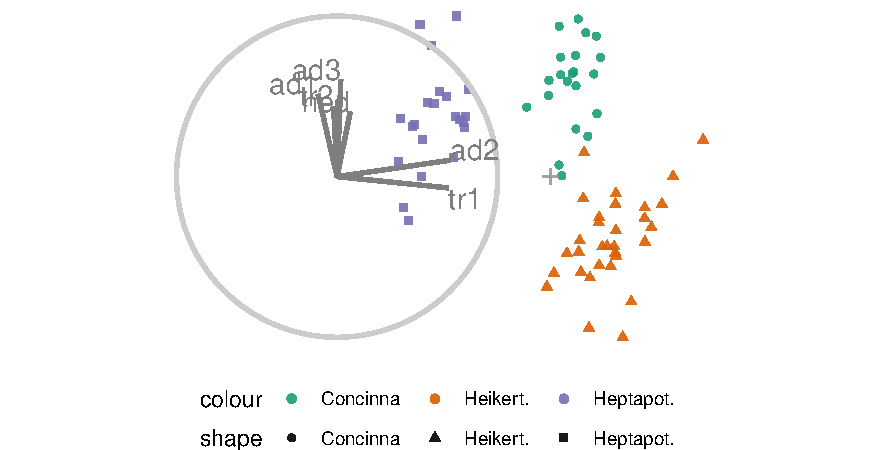
\includegraphics[width=1\linewidth,]{./figures_from_script/ch3_fig1_biplot} 

}

\caption{<a figure caption> XXX: TODO}\label{fig:ch3fig1}
\end{figure}

\begin{figure}

{\centering 
\includegraphics[width=1\linewidth,]{./figures_from_script/ch3_fig2_manip_sp} 

}

\caption{<a figure caption> XXX: TODO}\label{fig:ch3fig2}
\end{figure}

\begin{figure}

{\centering 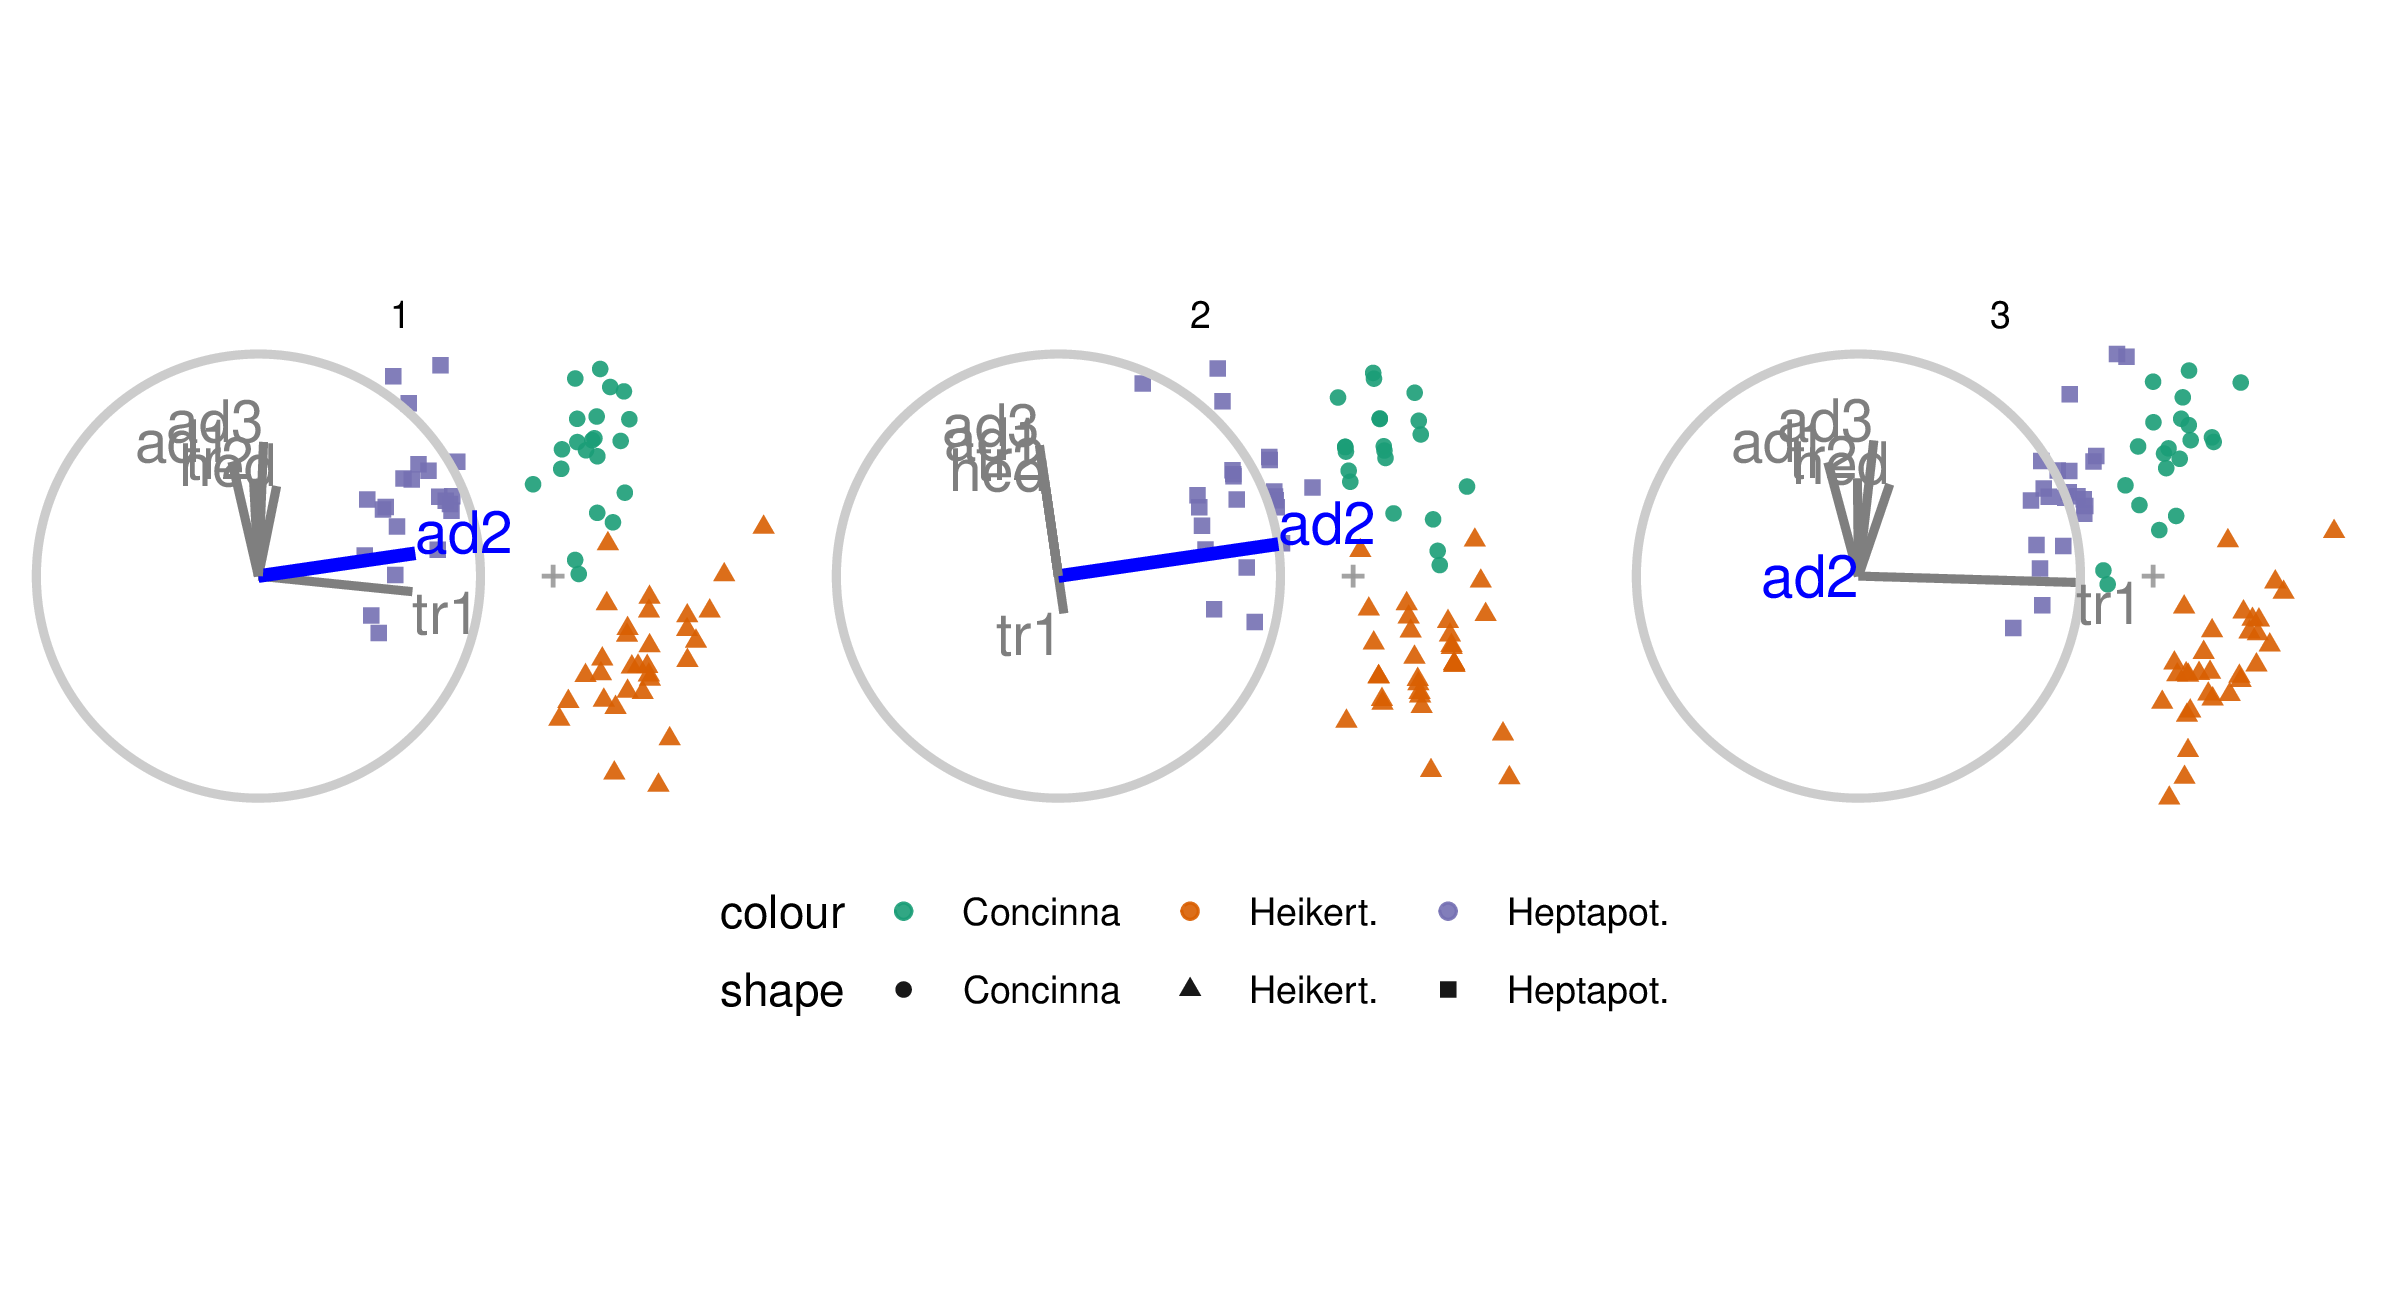
\includegraphics[width=1\linewidth,]{./figures_from_script/ch3_fig3_filmstrip} 

}

\caption{<a figure caption> XXX: TODO}\label{fig:ch3fig3}
\end{figure}

\begin{figure}

{\centering 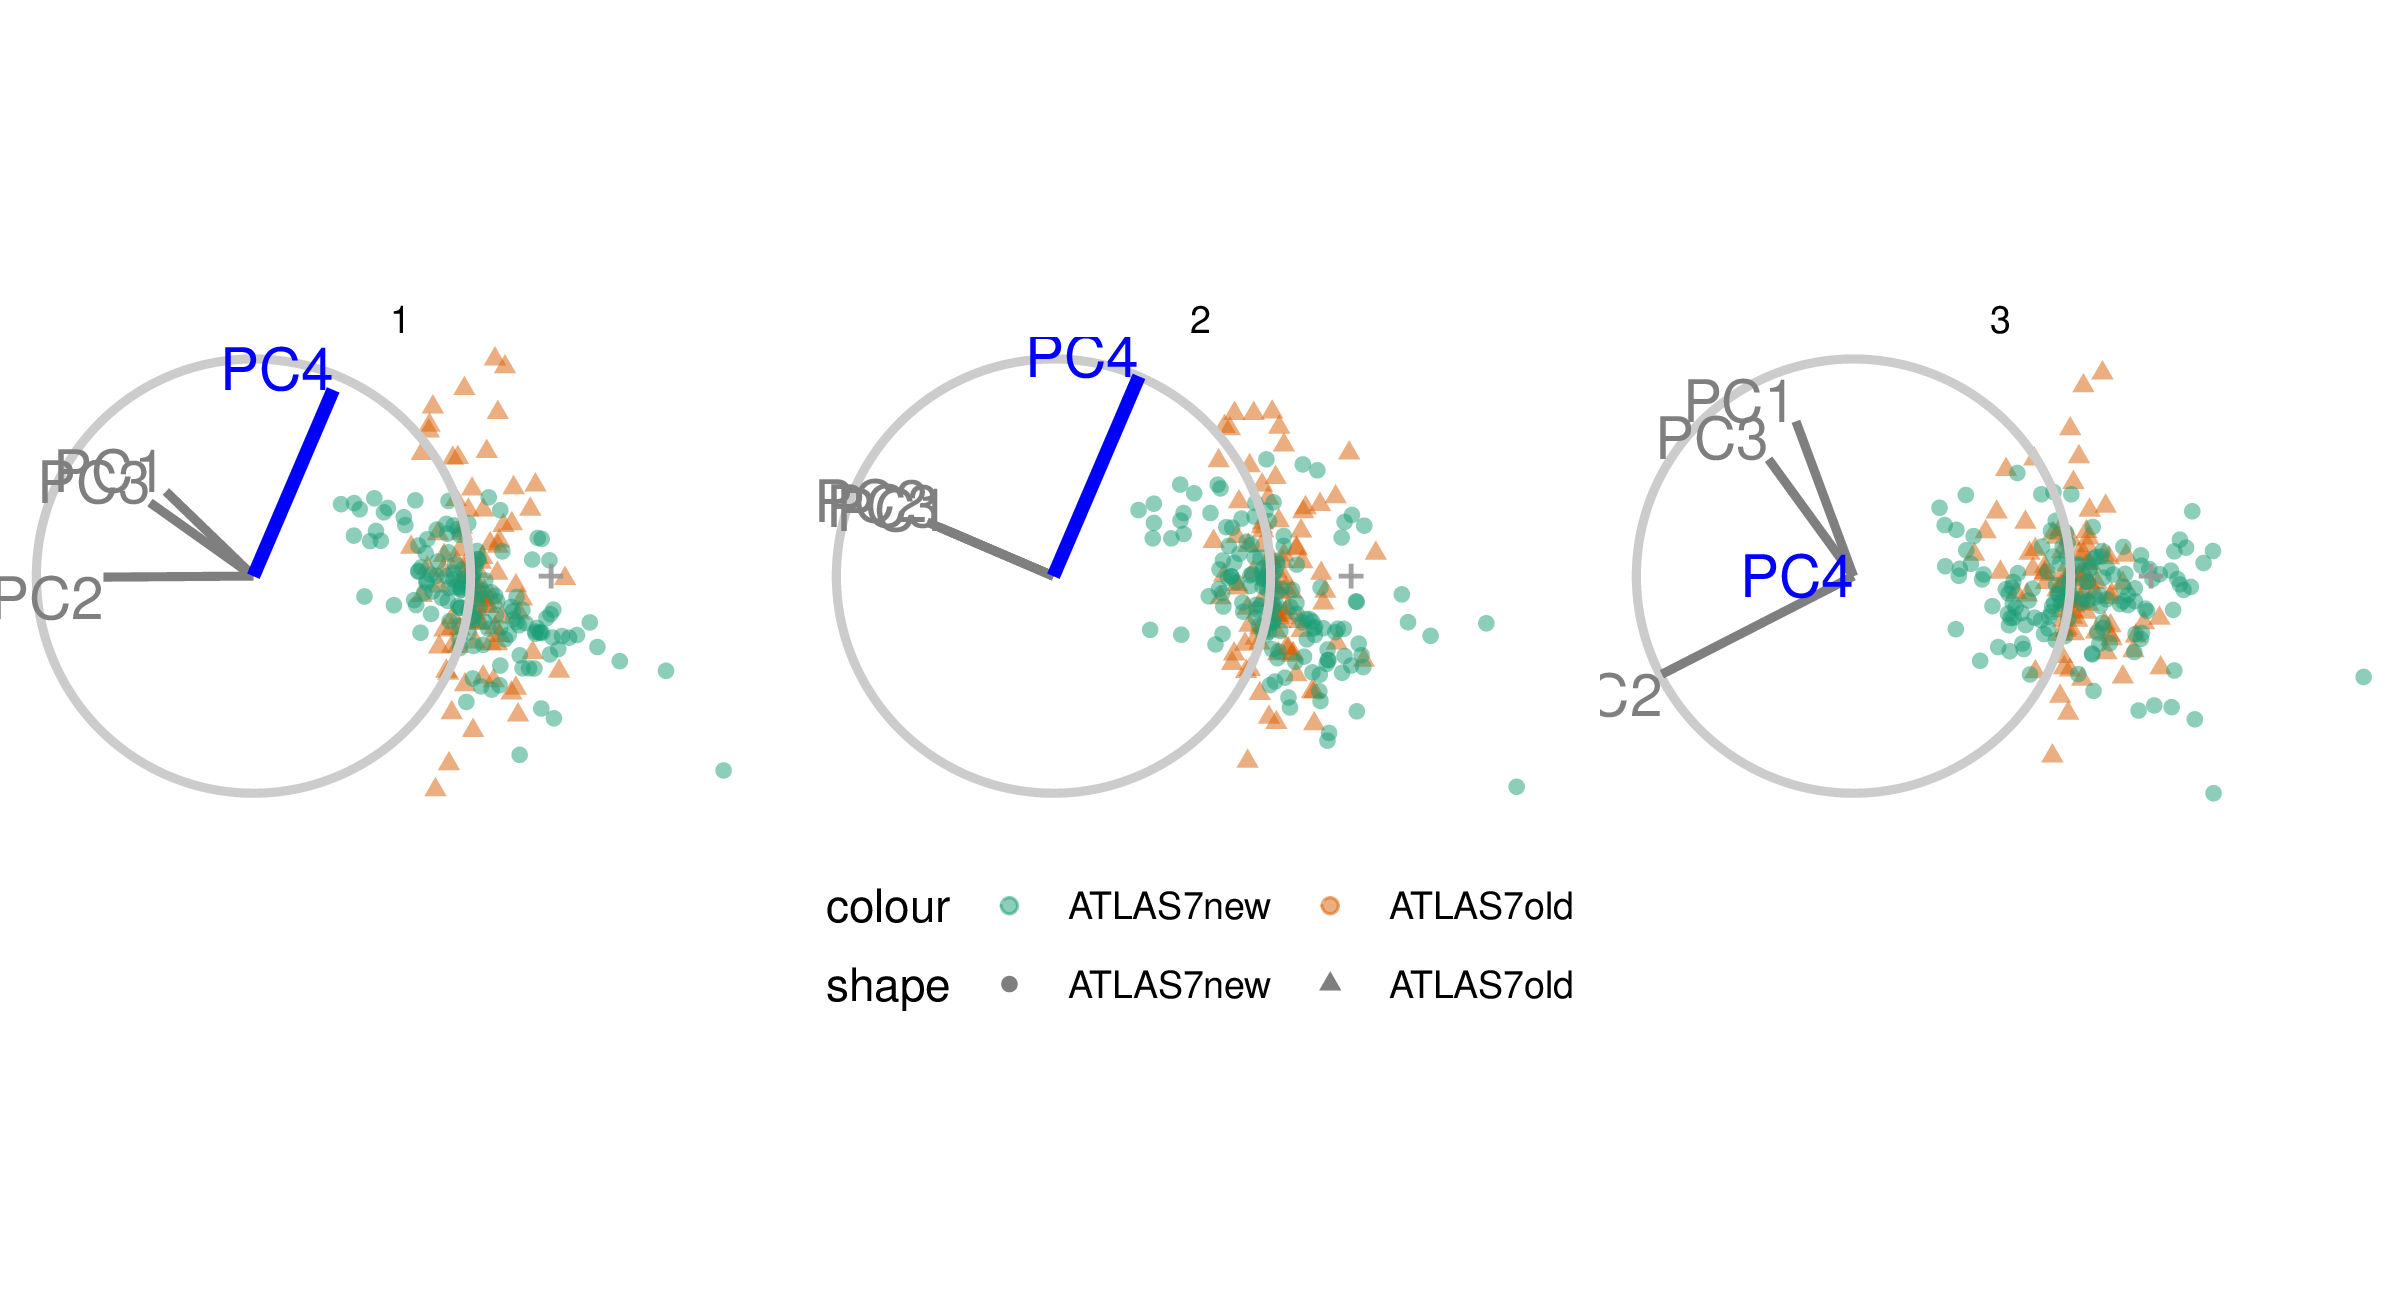
\includegraphics[width=1\linewidth,]{./figures_from_script/ch3_fig4_jet_better_pc4} 

}

\caption{<a figure caption> XXX: TODO}\label{fig:ch3fig4}
\end{figure}

\begin{figure}

{\centering 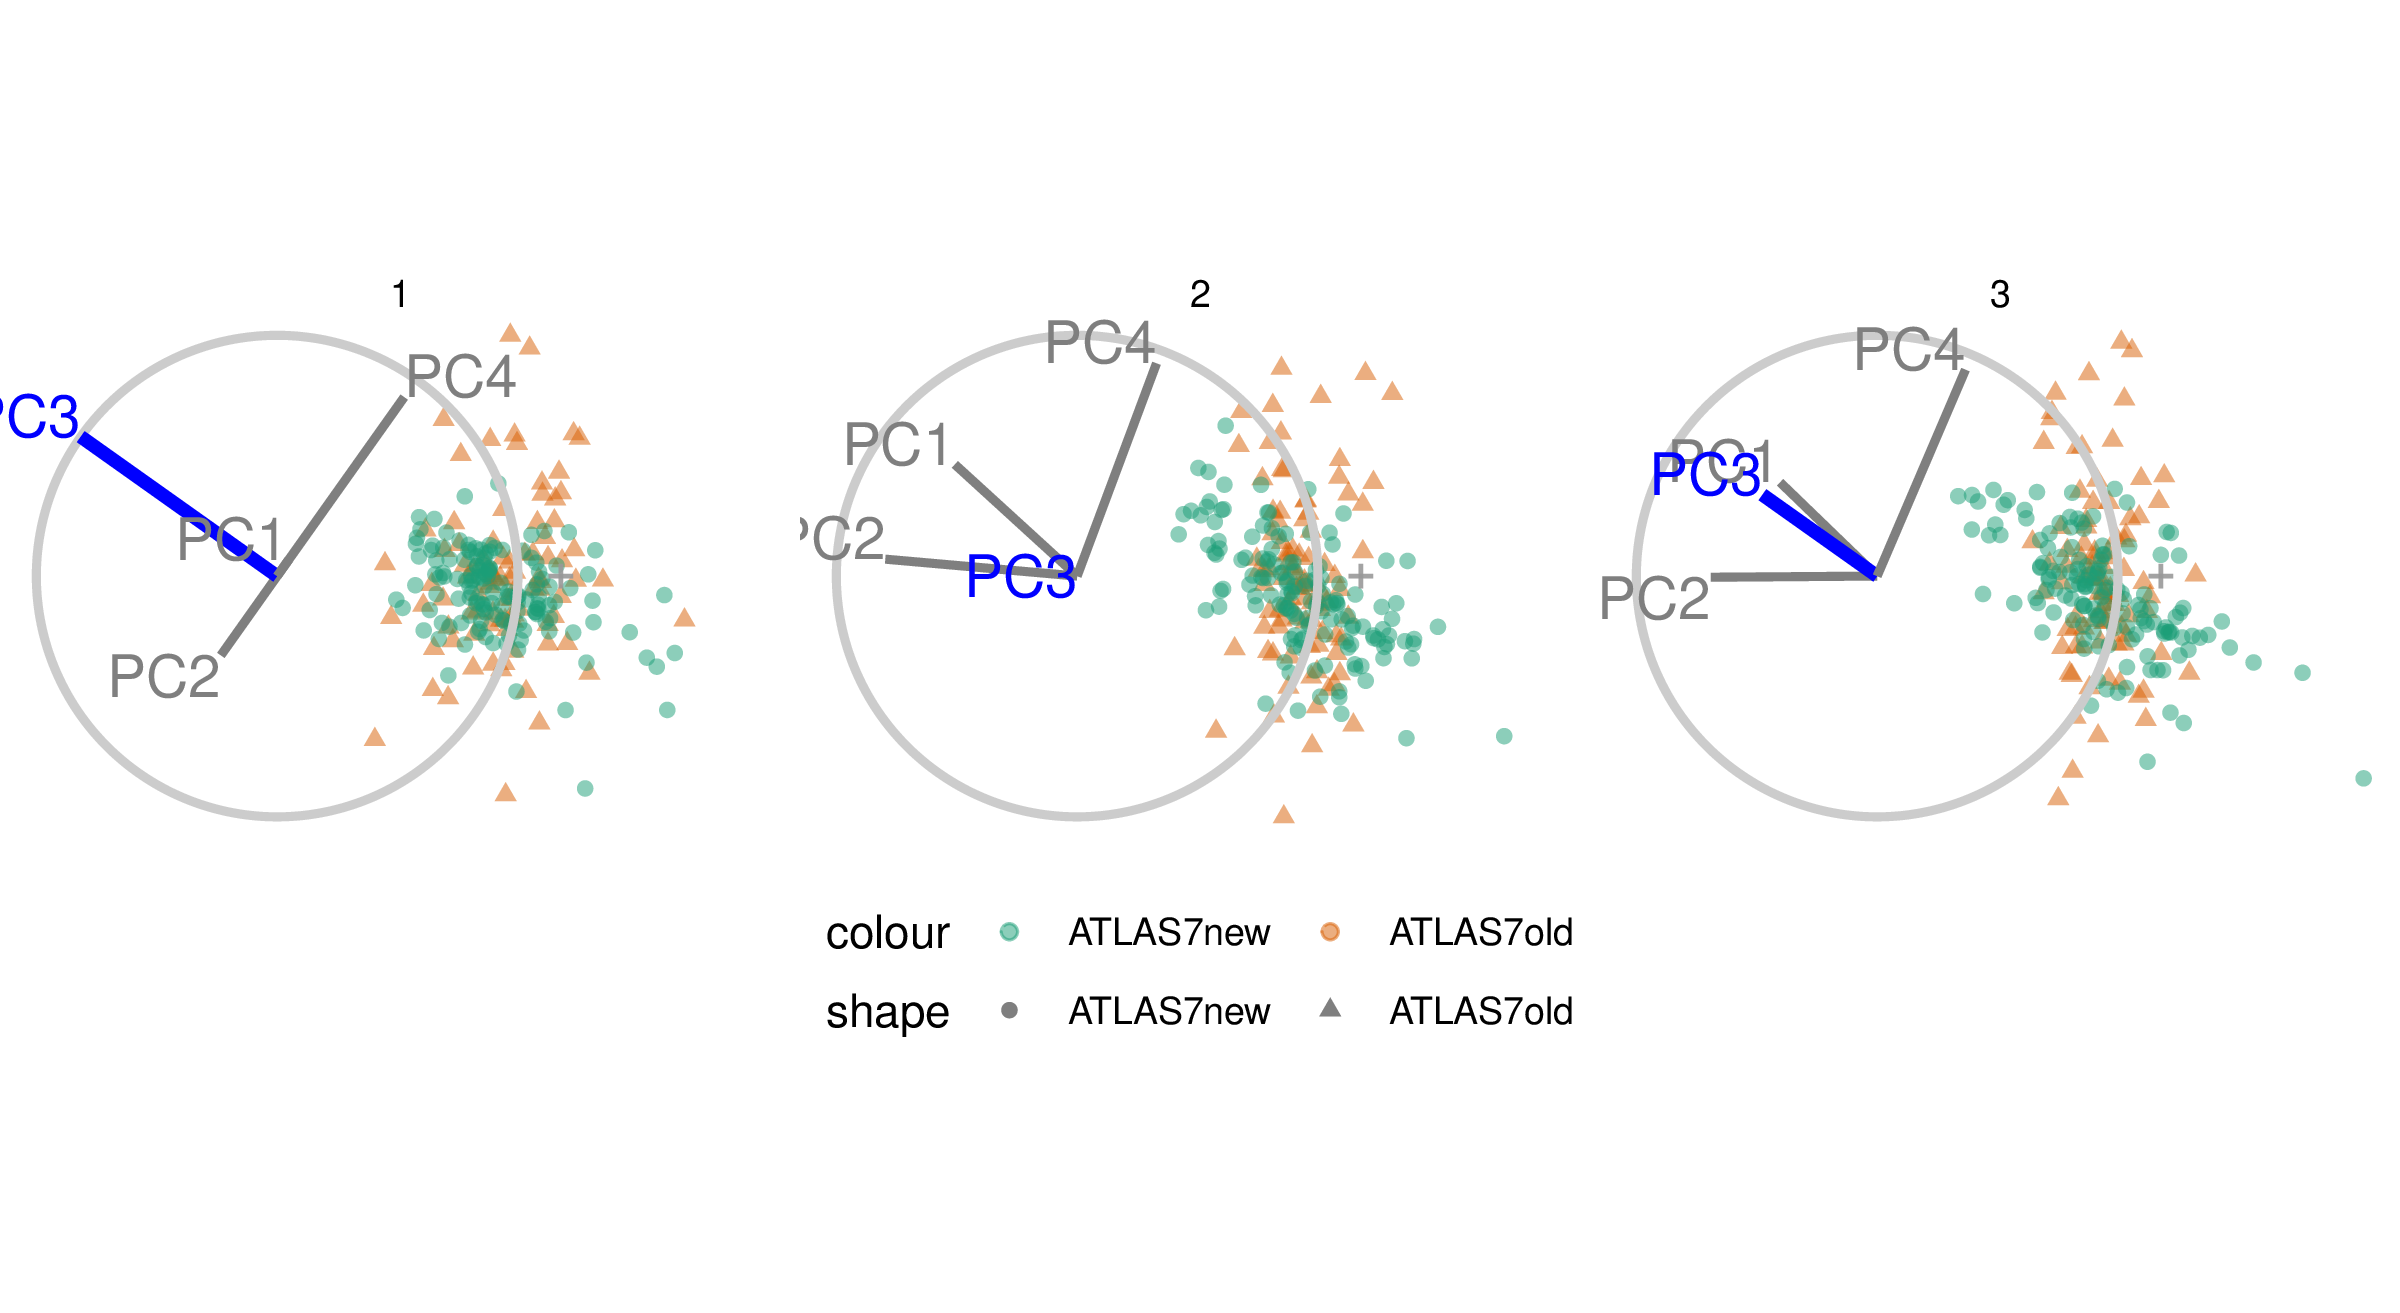
\includegraphics[width=1\linewidth,]{./figures_from_script/ch3_fig5_jet_worse_pc3} 

}

\caption{<a figure caption> XXX: TODO}\label{fig:ch3fig5}
\end{figure}

\begin{figure}

{\centering 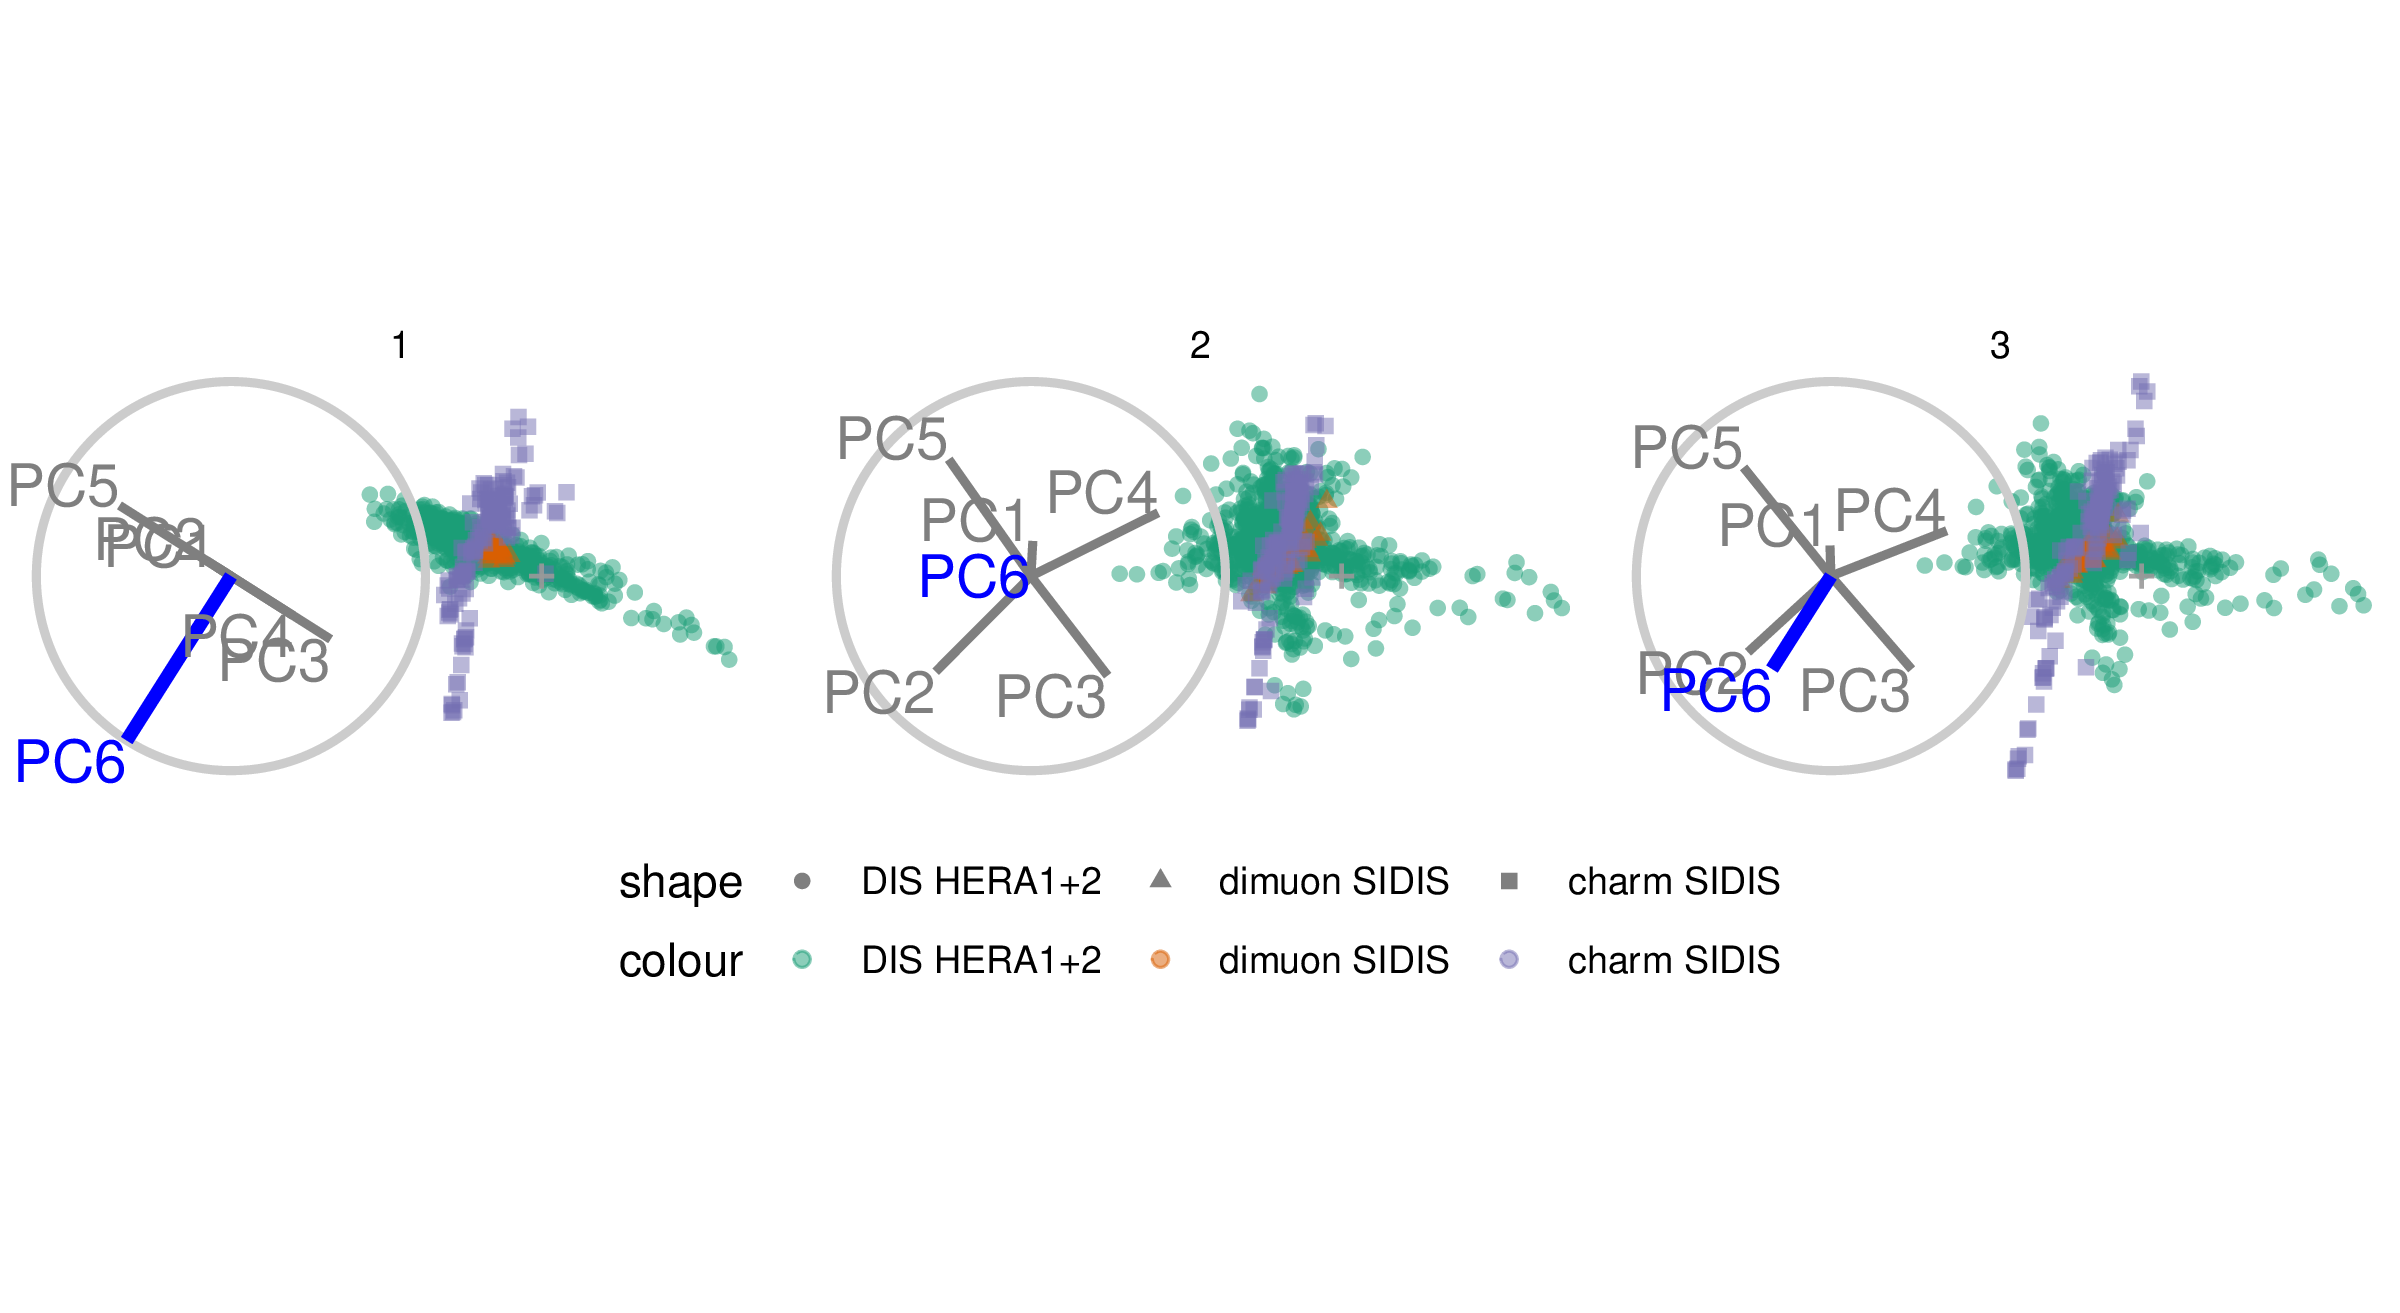
\includegraphics[width=1\linewidth,]{./figures_from_script/ch3_fig6_DIS_better_pc6} 

}

\caption{<a figure caption> XXX: TODO}\label{fig:ch3fig6}
\end{figure}

\begin{figure}

{\centering 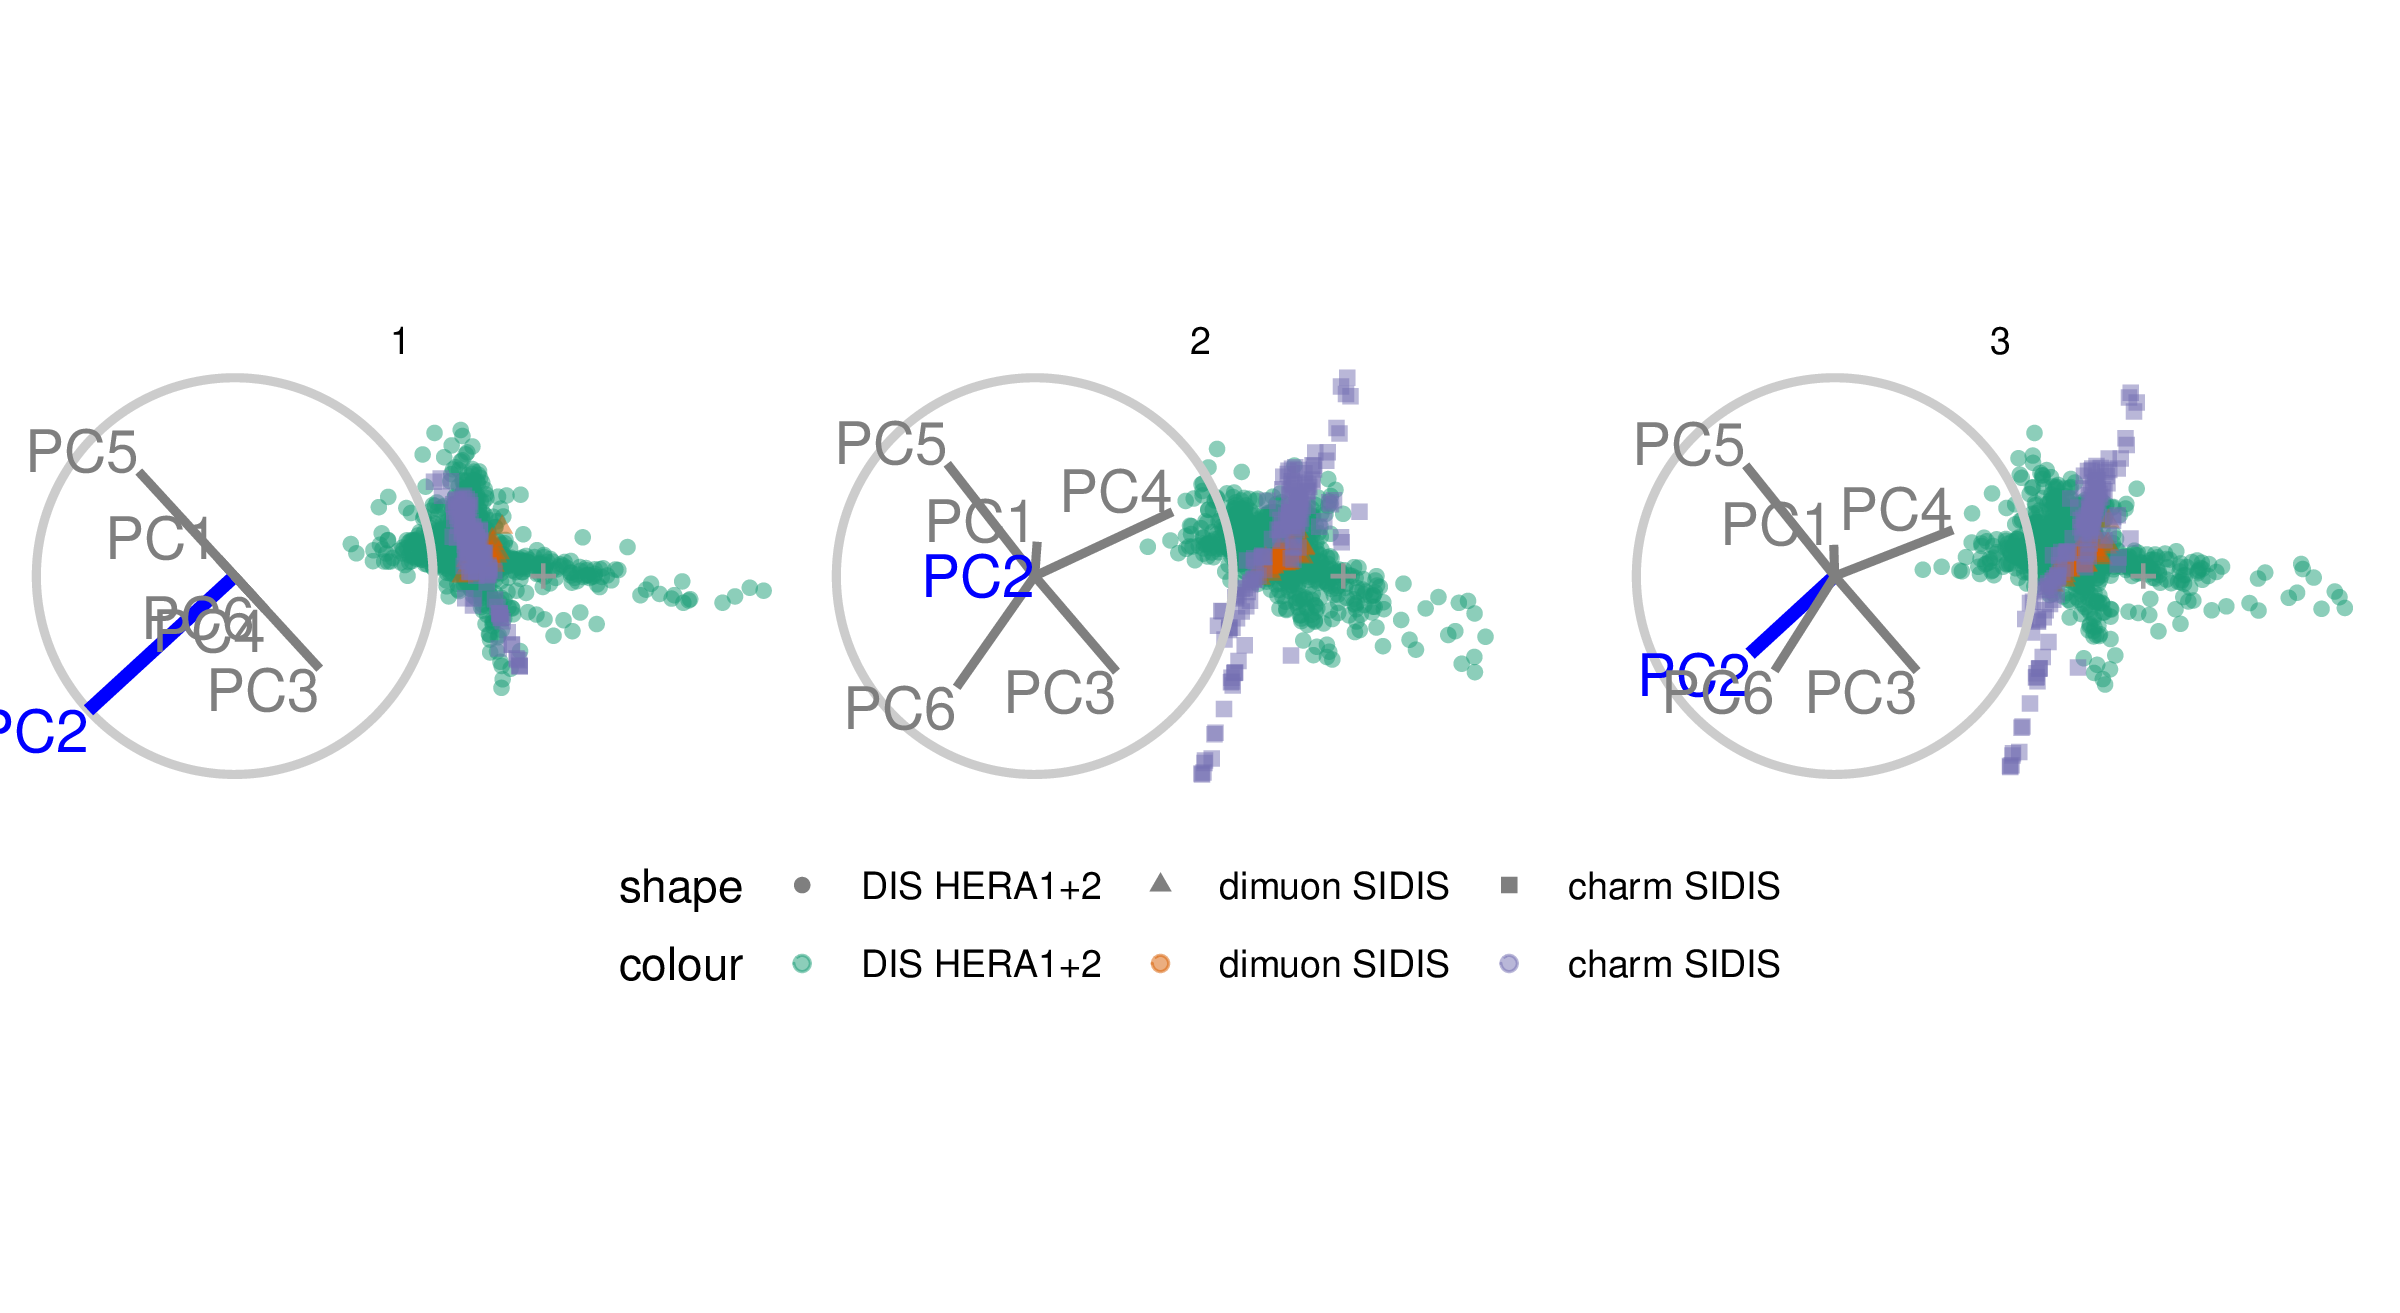
\includegraphics[width=1\linewidth,]{./figures_from_script/ch3_fig7_DIS_worse_pc2} 

}

\caption{<a figure caption> XXX: TODO}\label{fig:ch3fig7}
\end{figure}

\hypertarget{ch:efficacy_radial_tour}{%
\chapter{Efficacy of the radial tour}\label{ch:efficacy_radial_tour}}

\begin{figure}

{\centering 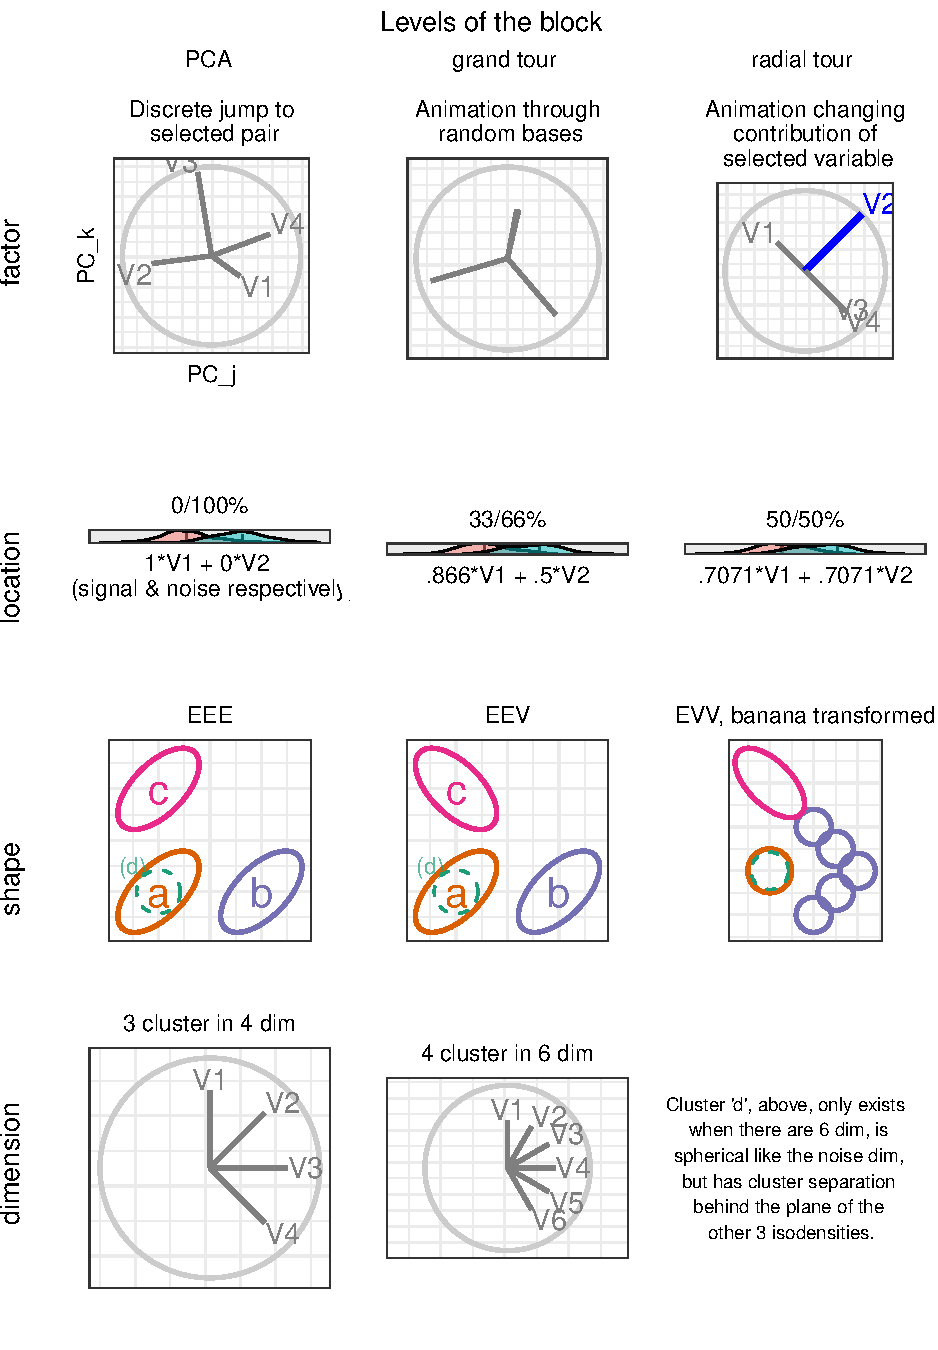
\includegraphics[width=1\linewidth,]{./figures_from_script/ch4_fig2_exp_factors} 

}

\caption{<a figure caption> XXX: TODO}\label{fig:ch4fig2}
\end{figure}

\begin{align*}
W_{j} &=\frac
{(\overline{X_{j=1, k=1}} - \overline{X_{1, k=2}}, ~...~
(\overline{X_{j=p, k=1}} - \overline{X_{j=p, k=2}})}
{\sum_{j=1}^{p}(|\overline{X_{j,k=1}} - \overline{X_{j,k=2}}|)}
- \frac{1}{p} \\
\\
\text{Accuracy}, Y &= \sum_{j=1}^{p}I(r_j) * sign(w_j) * \sqrt{|w_j|}  \\
\end{align*}

\begin{figure}

{\centering 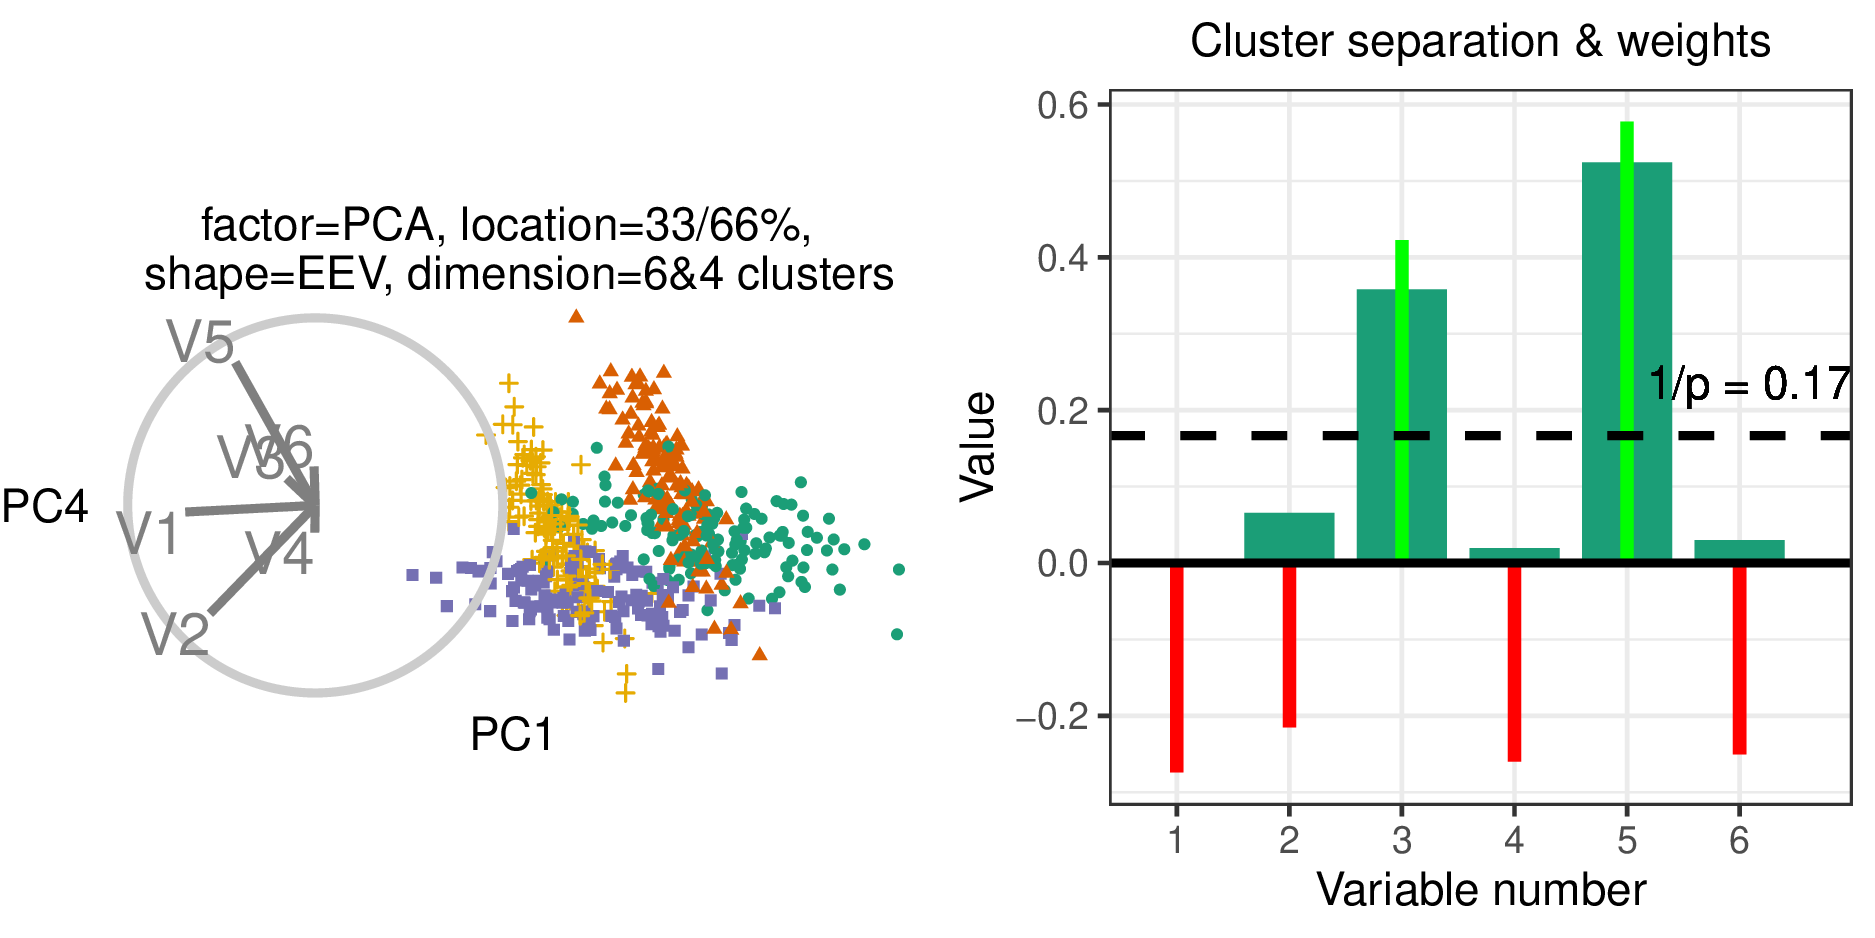
\includegraphics[width=1\linewidth,]{./figures_from_script/ch4_fig3_accuracy_measure} 

}

\caption{<a figure caption> XXX: TODO}\label{fig:ch4fig3}
\end{figure}

\[
\begin{array}{ll}
\textbf{Fixed effects:}          &\textbf{Full model:} \\
\alpha                           &\widehat{Y_1} = \mu + \alpha_i + \textbf{Z} + \textbf{W} + \epsilon \\
\alpha + \beta + \gamma + \delta &\widehat{Y_1} = \mu + \alpha_i + \beta_j + \gamma_k + \delta_l + \textbf{Z} + \textbf{W} + \epsilon \\
\alpha * \beta + \gamma + \delta &\widehat{Y_1} = \mu + \alpha_i * \beta_j + \textbf{Z} + \textbf{W} + \epsilon \\
\alpha * \beta * \gamma + \delta &\widehat{Y_1} = \mu + \alpha_i * \beta_j * \gamma_k + \textbf{Z} + \textbf{W} + \epsilon \\
\alpha * \beta * \gamma * \delta &\widehat{Y_1} = \mu + \alpha_i * \beta_j * \gamma_k * \delta_l + \textbf{Z} + \textbf{W} + \epsilon
\% \end{array}
\% \]
\% \[
\% \begin{array}{ll}
\text{where } &\mu \text{ is the intercept of the model including the mean of random effect} \\
&\alpha_i \text{, fixed term for factor}~|~i\in (\text{pca, grand, radial}) \\
&\beta_j  \text{, fixed term for location}~|~j\in (\text{0\_1, 33\_66, 50\_50}) \text{ \% noise/signal mixing} \\
&\gamma_k \text{, fixed term for shape}~|~k\in (\text{EEE, EEV, EVV banana}) \text{ model shapes} \\
&\delta_l \text{, fixed term for dimension}~|~l\in (\text{4 variables \& 3 cluster, 6 variables \& 4 clusters}) \\
&\textbf{Z} \sim \mathcal{N}(0,~\tau), \text{ the random effect of participant} \\
&\textbf{W} \sim \mathcal{N}(0,~\upsilon), \text{ the random effect of simulation} \\
&\epsilon   \sim \mathcal{N}(0,~\sigma), \text{ the error of the model} \\
\end{array}
\]

\begin{verbatim}
$ABcd_coef
                     Estimate Std. Error    df t value Pr(>|t|)    
(Intercept)             -0.12       0.08  43.9   -1.50     0.14    
fct=grand                0.15       0.09 622.4    1.74     0.08    
fct=radial               0.37       0.09 617.1    4.18     0.00 ***
loc=33_66                0.17       0.09  83.2    1.78     0.08    
loc=50_50                0.14       0.09  84.8    1.52     0.13    
shp=EEV                  0.04       0.06  11.5    0.79     0.44    
shp=ban                 -0.03       0.06  11.5   -0.48     0.64    
dim=6                   -0.06       0.05  11.5   -1.39     0.19    
fct=grand:loc=33_66     -0.06       0.13 587.3   -0.49     0.63    
fct=radial:loc=33_66    -0.34       0.13 585.2   -2.65     0.01  **
fct=grand:loc=50_50     -0.09       0.13 589.6   -0.68     0.50    
fct=radial:loc=50_50    -0.19       0.13 574.3   -1.43     0.15    

$t_ABcd_coef
                     Estimate Std. Error    df t value Pr(>|t|)    
(Intercept)              2.71       0.14  42.6   19.06     0.00 ***
fct=grand               -0.23       0.12 567.6   -1.97     0.05   *
fct=radial               0.16       0.12 573.5    1.34     0.18    
loc=33_66                0.05       0.14  40.9    0.34     0.74    
loc=50_50               -0.05       0.14  42.1   -0.35     0.73    
shp=EEV                 -0.15       0.09   8.3   -1.61     0.14    
shp=ban                 -0.13       0.09   8.3   -1.42     0.19    
dim=6                    0.14       0.08   8.3    1.90     0.09    
fct=grand:loc=33_66      0.24       0.18 580.9    1.34     0.18    
fct=radial:loc=33_66    -0.24       0.18 582.4   -1.32     0.19    
fct=grand:loc=50_50      0.12       0.18 578.6    0.69     0.49    
fct=radial:loc=50_50     0.05       0.18 584.4    0.25     0.80    
List of 2
 $ ABcd_coef  :'data.frame':    12 obs. of  6 variables:
  ..$ Estimate  : num [1:12] -0.12 0.15 0.37 0.17 0.14 0.04 -0.03 -0.06 -0.06 -0.34 ...
  ..$ Std. Error: num [1:12] 0.08 0.09 0.09 0.09 0.09 0.06 0.06 0.05 0.13 0.13 ...
  ..$ df        : num [1:12] 43.9 622.4 617.1 83.2 84.8 ...
  ..$ t value   : num [1:12] -1.5 1.74 4.18 1.78 1.52 0.79 -0.48 -1.39 -0.49 -2.65 ...
  ..$ Pr(>|t|)  : num [1:12] 0.14 0.08 0 0.08 0.13 0.44 0.64 0.19 0.63 0.01 ...
  ..$           : chr [1:12] "" "" "***" "" ...
 $ t_ABcd_coef:'data.frame':    12 obs. of  6 variables:
  ..$ Estimate  : num [1:12] 2.71 -0.23 0.16 0.05 -0.05 -0.15 -0.13 0.14 0.24 -0.24 ...
  ..$ Std. Error: num [1:12] 0.14 0.12 0.12 0.14 0.14 0.09 0.09 0.08 0.18 0.18 ...
  ..$ df        : num [1:12] 42.6 567.6 573.5 40.9 42.1 ...
  ..$ t value   : num [1:12] 19.06 -1.97 1.34 0.34 -0.35 ...
  ..$ Pr(>|t|)  : num [1:12] 0 0.05 0.18 0.74 0.73 0.14 0.19 0.09 0.18 0.19 ...
  ..$           : chr [1:12] "***" "*" "" "" ...
\end{verbatim}

\begin{figure}

{\centering 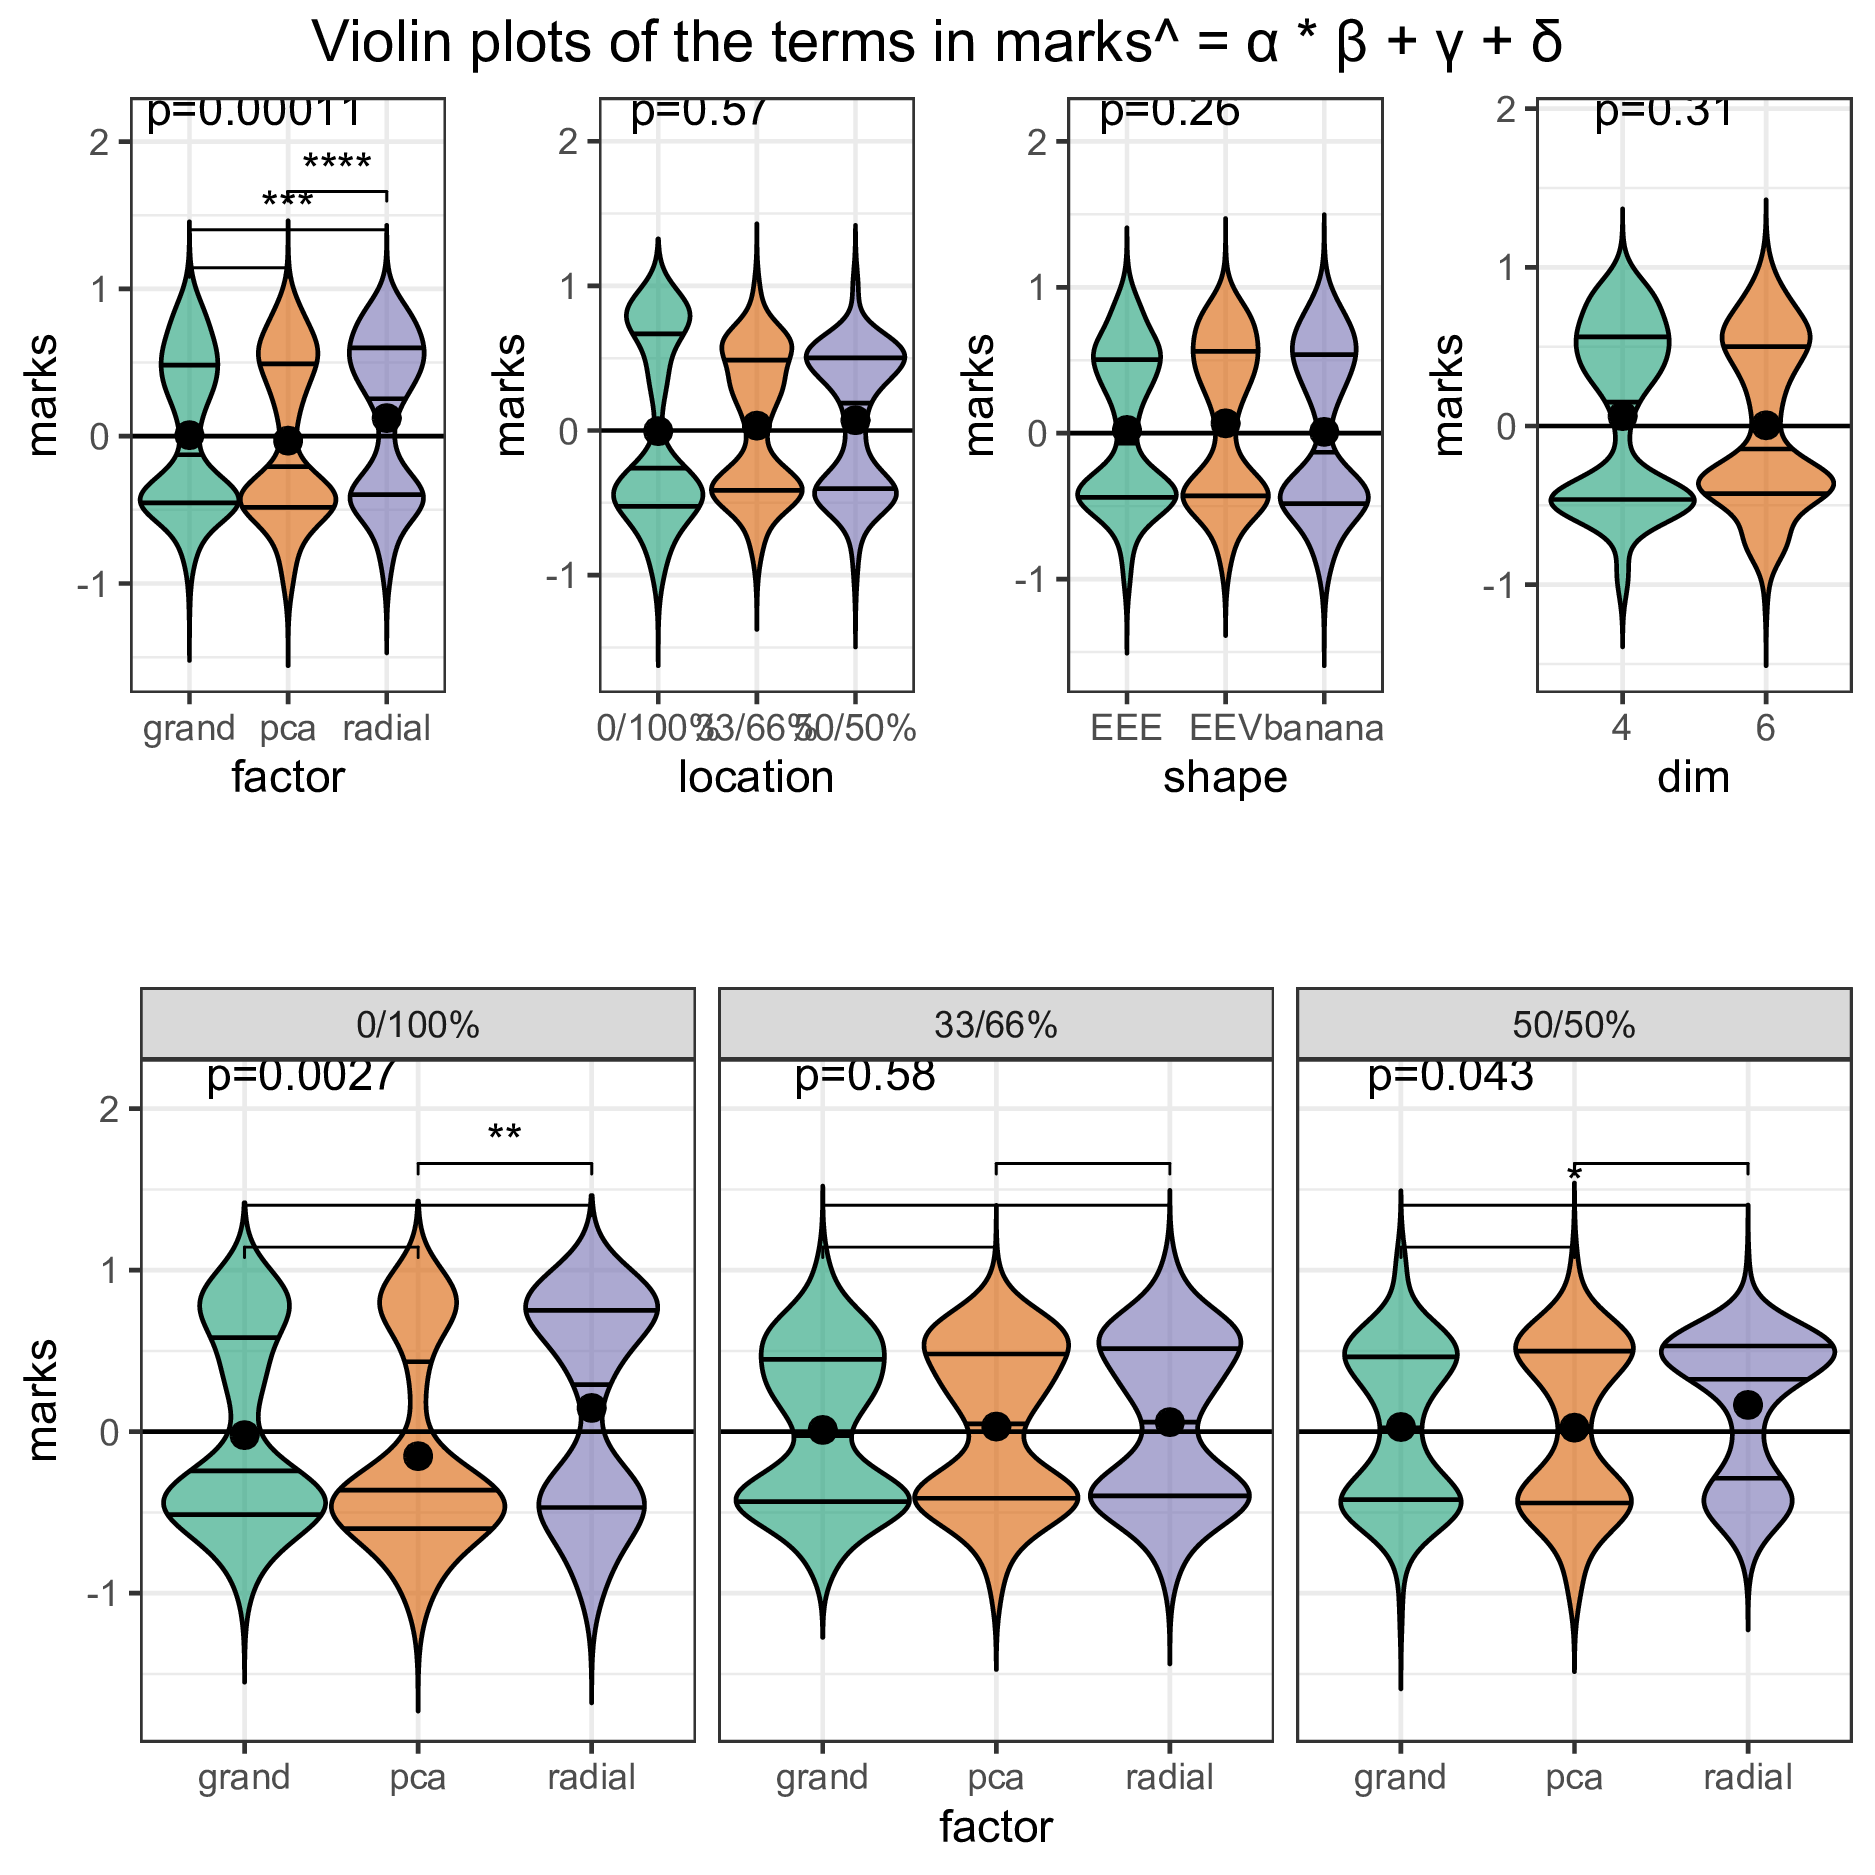
\includegraphics[width=1\linewidth,]{./figures_from_script/ch4_fig5_ABcd_violins} 

}

\caption{<a figure caption> XXX: TODO}\label{fig:ch4fig5}
\end{figure}

\begin{figure}

{\centering 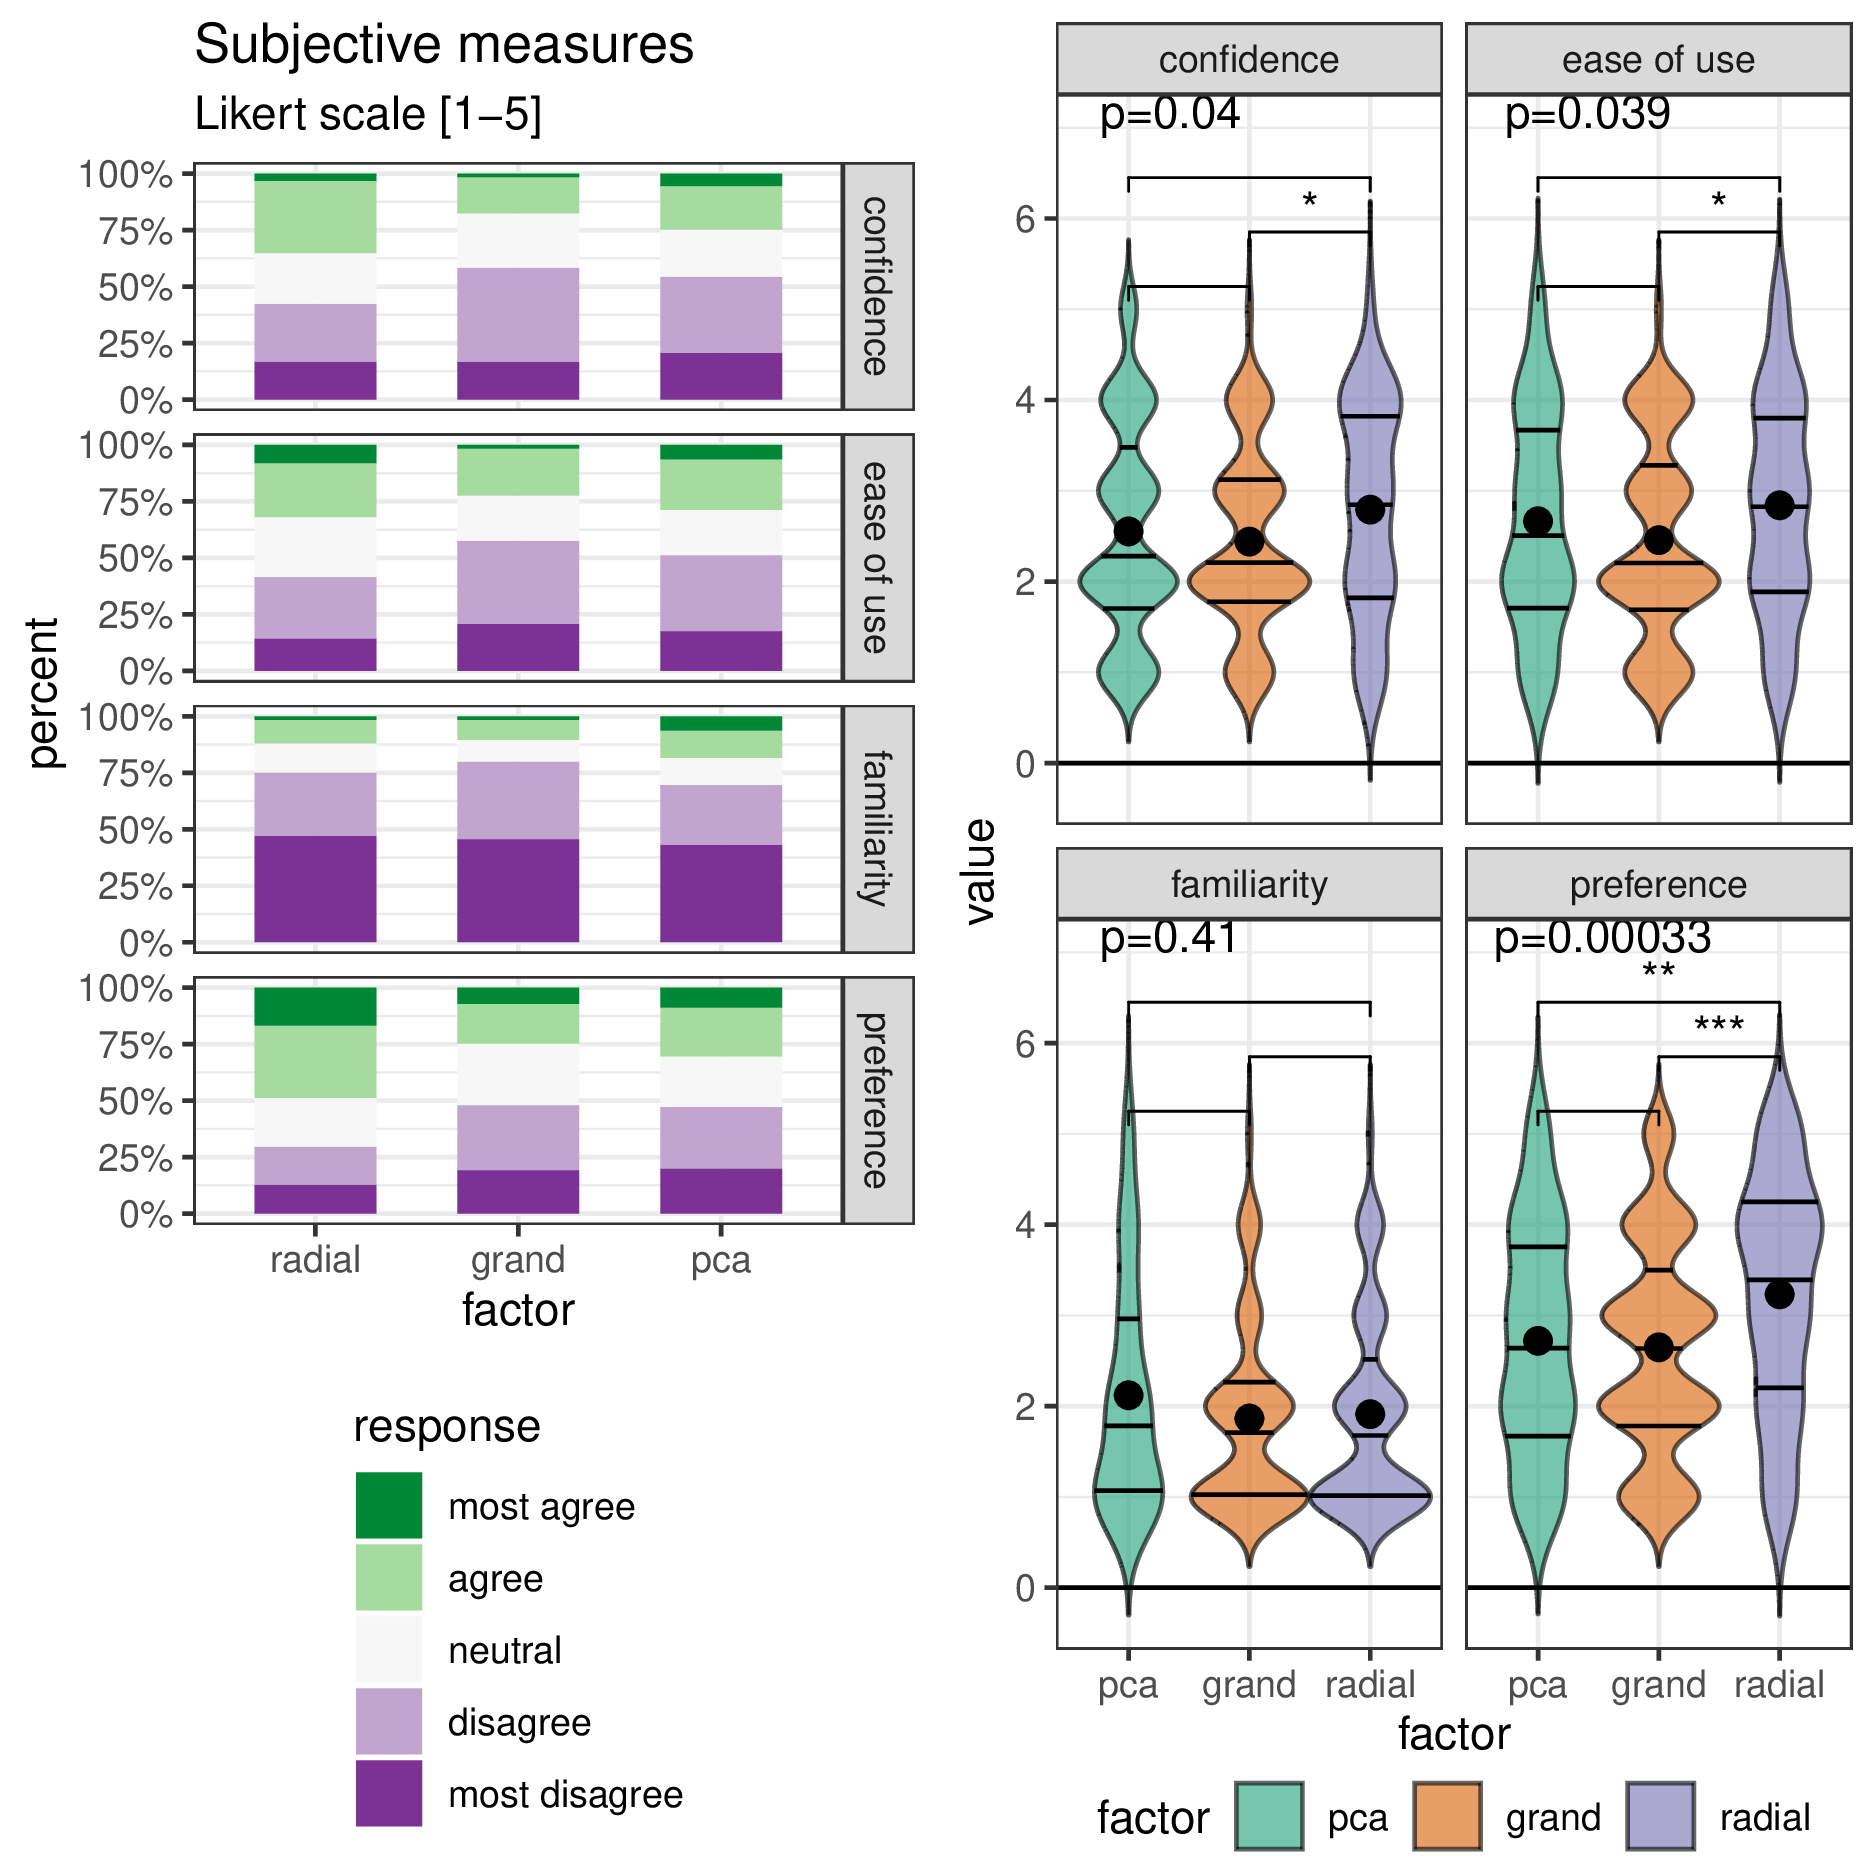
\includegraphics[width=1\linewidth,]{./figures_from_script/ch4_fig6_subjective_measures} 

}

\caption{<a figure caption> XXX: TODO}\label{fig:ch4fig6}
\end{figure}

\printbibliography[heading=bibintoc]



\end{document}
